\chapter{Physical Properties for Audio Sound Generated by a PAL} % Main chapter title
\label{chap:phys} % Change X to a consecutive number; for referencing this chapter elsewhere, use \ref{ChapterX}

\blfootnote{The work presented in this chapter have been published in \cite{Zhong2020InsertionLossThin, Zhong2020ReflectionAudioSounds, Zhong2022ScatteringRigidSphere}.}

\noindent This chapter focuses on the investigation of the physical properties for audio sound generated by a PAL.
Section \ref{sec:phys_reflection} investigates the reflection from an infinitely large surface.
Section \ref{sec:phys_transmission} investigates the transmission through a thin partition and a model for calculating the insertion loss.
Section \ref{sec:phys_scat} investigates the scattering by a rigid sphere which simulates a human head in applications.



\section{Reflection from an infinitely large surface}
\label{sec:phys_reflection}
Existing analytical models of the PAL consider the sound radiation in free space, but do not pay much attention to its reflection, which is important in many applications \cite{HolosonicsResearchLabs2016UserManualAudio}.
For example, PALs have been used to measure the sound absorption coefficients of materials in air \cite{Castagnede2008LowFrequencySitu, Sugahara2019MeasurementsAcousticImpedance, Romanova2019ApplicationParametricTransducer}
and the reflection and transmission coefficients of elastomeric materials underwater \cite{Humphrey1985MeasurementAcousticProperties, Humphrey2008AcousticCharacterizationPanel}
and to actively control the binaural noise at human ears \cite{Tanaka2017BinauralActiveNoise} where the reflection happens on the material surface or human skin and hair.

When there is a reflecting surface near a PAL, both primary and secondary sound waves are reflected by the surface. 
The reflection by a pressure-release surface has been studied for underwater applications \cite{Muir1977ReflectionFiniteAmplitude}.
This model assumes that the primary fields are plane waves within the Rayleigh distance and spherical waves afterwards, and the analysis is based on the weak shock wave theory. 
It was found that the DFW generated by the incident primary waves is anti-phase with itself after the pressure-release reflection, while the DFW generated by the reflected primary waves is in-phase with the incident DFW. 
Therefore, the DFW suffers from a phase cancellation effect and this phenomenon has been observed in experiments \cite{Muir1977ReflectionFiniteAmplitude}.
The studies were then extended to the finite size planar targets with the weak nonlinearity by using a more accurate model {using the KZK equation} \cite{Garrett1984ReflectionParametricRadiation}.

The reflection of the water-air (pressure-release) interface with a small grazing angle was modeled to investigate its effects on acoustic communication in shallow-water channels \cite{Wang1999SecondaryFieldParametric}.
Two theoretical models were proposed: a simplified Westervelt model where the primary waves are highly attenuated within the collimated zone, and a spherical spreading model where the interaction of primary waves is significant in the far field spherically spreading beam. 
Experiments were conducted at $5.4^\circ$ and $7.7^\circ$ grazing angles and only the spherical spreading model was shown to agree well with experiment. 

Except for the experimental studies conducted underwater in the aforementioned literatures, the reflection of audio sound generated by a PAL in air has also been studied experimentally \cite{Pompei2002SoundUltrasoundParametric}.
It was found that the sound reflected from a rigid wall maintain the same directivity as the incident beam, but those reflected from a wall covered with a diffusive panel lose the directivity completely. 
However, the effects of the reflection of ultrasound were not considered in this research \cite{Pompei2002SoundUltrasoundParametric}. 
When a PAL radiates sound in air in the presence of a reflecting surface, additional audio sound components are generated by the reflected ultrasound waves. 
The two models proposed in \cite{Wang1999SecondaryFieldParametric} are only valid in the far field while the model in \cite{Garrett1984ReflectionParametricRadiation} is valid in the near-field but limited to the paraxial region. 
The non-paraxial model in \cite{Cervenka2013NonparaxialModelParametric, Zhong2020SphericalExpansionAudio} is more accurate at wide-angle field but has not considered reflections. 
In this section, the non-paraxial model is extended to investigate the reflection of audio sound generated by a PAL. 
Simulations are carried out for oblique incident sound first, and then the experimental results are presented to verify the findings.


\subsection{Theory}
As shown in Fig.~\ref{fig:reflection_sketch}(a), assume a PAL in free field generates two harmonic ultrasound at frequencies $f_1$ and $f_2$  with the boundary condition on the transducer surface given by Eq.~(\ref{eq:velocity_condition_3d}).
\revA{The audio sound generated by the nonlinear interactions of ultrasound is equivalent to the radiation from a virtual source within an infinitely large volume, where the source density is proportional to the ultrasound field.}
Fig.~\ref{fig:reflection_sketch}(b) shows a PAL radiating ultrasound to an infinitely large reflecting surface with an incident angle $\theta$, where the distance between the PAL center and the reflecting surface is $D$, and the origin of the coordinate system, $O$, is set at the projection point of the PAL on the reflecting surface with the positive $z$ axis pointing to the center of the PAL. 
When the sound beams impinge on the reflecting surface, both ultrasound and audio sound are reflected. 
The total audio sound mainly consists of four components as shown in Fig.~\ref{fig:reflection_sketch}(b), and can be expressed as
\begin{equation}
    \Phi\subt{tot}(\vb{r}, k\subt{a}) 
    = \Phi\subt{inc,+}(\vb{r}, k\subt{a})
    + \Phi\subt{inc,-} (\vb{r}, k\subt{a}) 
    + \Phi\subt{refl,+} (\vb{r}, k\subt{a})
    + \Phi\subt{refl,-} (\vb{r}, k\subt{a})
    \label{eq:reflection_component}
\end{equation}
where $\Phi\subt{inc,+}$ is generated by the nonlinear interactions of incident ultrasound, $\Phi\subt{inc,-}$ is the reflection of $\Phi\subt{inc,+}$ to satisfy the boundary condition on the reflecting surface for audio sound,
$\Phi\subt{refl,+}$ is generated by the nonlinear interactions of reflected ultrasound, 
and $\Phi\subt{refl,-}$ is the reflection of $\Phi\subt{refl,+}$.
The corresponding sound pressure $p\subt{tot}, p\subt{inc,\pm}$, and $  p\subt{refl,\pm}$ can be obtained using Eq.~(\ref{eq:pressure_potential_linear}).
These four components will be analyzed individually in the following paragraphs.

\begin{figure}[!htb]
    \centering
    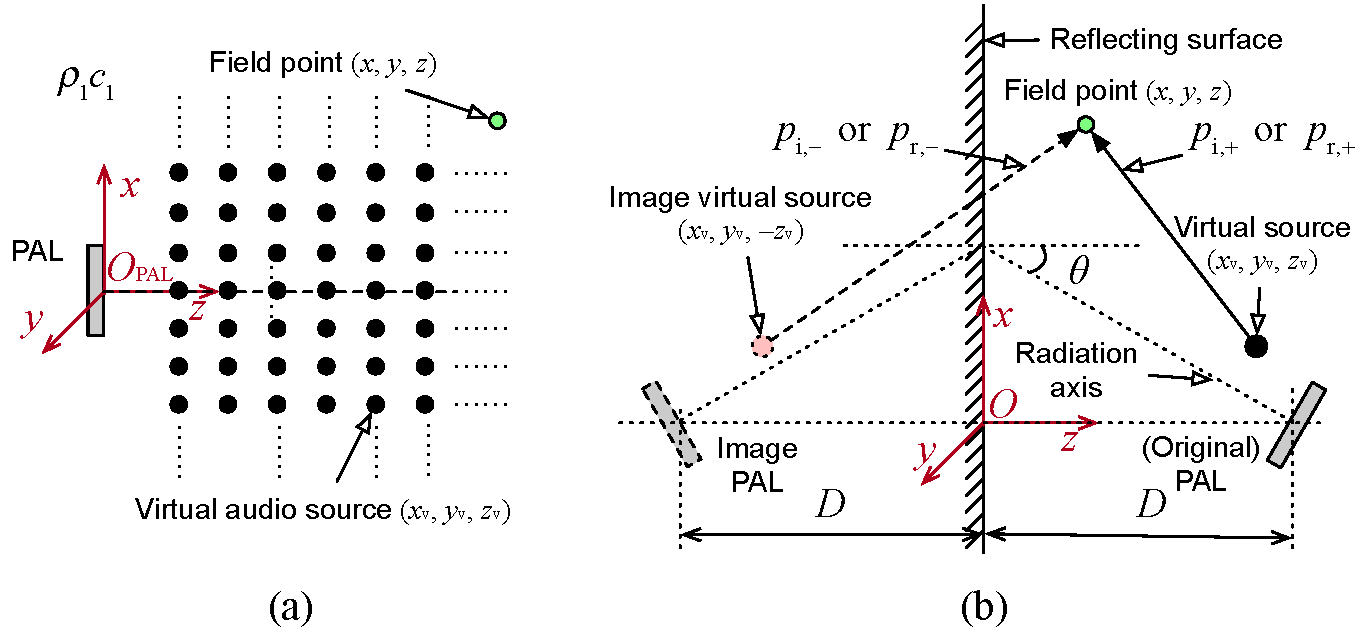
\includegraphics[width = 0.95\textwidth]{Figures/pending/Figure1_Reflection_Sketch.pdf}
    \caption{A PAL radiating sound (a) in free field or (b) to an infinitely large reflecting surface with an incident angle $\theta$.}
    \label{fig:reflection_sketch}
\end{figure}

It is noteworthy the nonlinear interactions of the incident and reflected ultrasound are neglected in this section because of the phase mismatching of the ultrasonic waves and small source density of the virtual source.
Further simulations show the audio sound generated by them is at least 35 dB less than that calculated by Eq.~(\ref{eq:reflection_component}) for the parameters used in this section, 
so they can be safely neglected to simplify the model and focus on the reflection phenomenon. 

The audio sound generated by the incident ultrasound is 
\begin{equation}
    \Phi\subt{inc,+}(\vb{r},k\subt{a})
    = -
    \int_0^\infty \int_{-\infty}^\infty \int_{-\infty}^\infty
    q\subt{inc}(\vb{r}\subt{v}) 
    g(\vb{r},\vb{r}\subt{v},k\subt{a})
    \dd^3 \vb{r}\subt{v}
    \label{eq:reflection_potential_inc_pos}
\end{equation}
where $|\vb{r}-\vb{r}\subt{v}| = \sqrt{(x-x\subt{v})^2 + (y-y\subt{v})^2 + (z-z\subt{v})^2}$ is the distance between the field point at $\vb{r}$ and the virtual source point at $\vb{r}\subt{v} = (x\subt{v},y\subt{v},z\subt{v})$.
The source density of the virtual source at $\vb{r}\subt{v}$ is given by 
\begin{equation}
    q\subt{inc} (\vb{r}\subt{v}) 
    = \frac{ \beta\omega\subt{a} \omega_1\omega2}{\rmi c_0^4}
    \Phi\subt{inc}(\vb{r}\subt{v}, k_1)
    \Phi\subt{inc}^*(\vb{r}\subt{v}, k_2)
\end{equation}
where the incident ultrasound $\Phi\subt{inc}(\vb{r}\subt{v}, k_i)$ is generated by the original PAL in free field at frequencies $f_i$. 

To satisfy the boundary condition on the reflecting surface for the audio sound $\Phi\subt{inc,+}$, the image for \revA{each virtual source at $\vb{r}\subt{v} = (x\subt{v}, y\subt{v} ,z\subt{v})$} is assumed to be at $\vb{r}\subt{v,-} = (x\subt{v}, y\subt{v}, -z\subt{v})$ with the source density $\scrR \subt{v} q\subt{inc}(\vb{r}\subt{v})$.
$R\subt{v}(\omega\subt{a})$ is the spherical wave reflection coefficient at frequency $f\subt{a}$, and it equals to 0 and 1 when the boundary is absolutely soft and rigid, respectively. 
For an arbitrary impedance boundary, $R\subt{v}(\omega\subt{a})$ depends on frequency, the source, and field point locations, as well as the incident angle and the admittance of the boundary \cite{Rudnick1947PropagationAcousticWave}.
The audio sound generated by the image virtual source is then obtained by 
\begin{equation}
    \Phi\subt{inc,-}(\vb{r},k\subt{a})
    = -
    \int_0^\infty \int_{-\infty}^\infty \int_{-\infty}^\infty
    \scrR\subt{v}(\omega\subt{a}) 
    q\subt{inc}(\vb{r}\subt{v}) 
    g(\vb{r},\vb{r}\subt{v,-},k\subt{a})
    \dd^3 \vb{r}\subt{v}
    \label{eq:reflection_potential_inc_minus}
\end{equation}
where $|\vb{r}-\vb{r}\subt{v,-}| = \sqrt{(x-x\subt{v})^2 + (y-y\subt{v})^2 + (z+z\subt{v})^2}$ is the distance between the field point at $\vb{r}$ and the image virtual source at $\vb{r}\subt{v,-}$.
It is noted that the spherical wave reflection coefficient is difficult to measure in experiments.
Because the audio beams generated by the PAL behave like plane waves (e.g., see \cite{Castagnede2008LowFrequencySitu}), the plane wave reflection coefficient can be used for simplicity.

The reflected ultrasound can be assumed to be the ultrasound generated by the same PAL at the position of its image position multiplied by a plane wave reflection coefficient $R(\omega_1)$ and $R(\omega_2)$ at frequencies $f_1$ and $f_2$, respectively.
The audio sound generated by the reflected ultrasound is then
\begin{equation}
    \Phi\subt{refl,+}(\vb{r},k\subt{a})
    = -
    \int_0^\infty \int_{-\infty}^\infty \int_{-\infty}^\infty
    \scrR(\omega_1)\scrR^*(\omega_2) q\subt{img}(\vb{r}\subt{v})
    g(\vb{r}, \vb{r}\subt{v},k\subt{a})
    \dd^3 \vb{r}\subt{v}
    \label{eq:reflection_potential_refl_pos}
\end{equation}
where the source density of the virtual source is 
\begin{equation}
    q\subt{img}(\vb{r}\subt{v})
    = \frac{ \beta \omega\subt{a}\omega_1\omega_2}{\rmi c_0^4}
    \Phi\subt{img}(\vb{r}\subt{v}, k_1)
    \Phi\subt{img}^*(\vb{r}\subt{v},k_2)
\end{equation}
and $\Phi\subt{img}(\vb{r}\subt{v}, k_1)$ and $\Phi\subt{img}(\vb{r}\subt{v},k_2)$ are the sound pressure for the corresponding ultrasound generated by the image PAL in free field at frequencies $f_1$ and $f_2$, respectively.
Similarly, to satisfy the boundary condition on the reflecting surface for audio sound, the reflection of $\Phi\subt{refl,+}$ is 
\begin{equation}
    \Phi\subt{refl,-}(\vb{r},k\subt{a})
    = -
    \int_0^\infty \int_{-\infty}^\infty \int_{-\infty}^\infty
    \scrR(\omega_1)
    \scrR^*(\omega_2) 
    \scrR\subt{v}(\omega\subt{a})
    q\subt{img}(\vb{r}\subt{v})
    g(\vb{r},\vb{r}\subt{v,-},k\subt{a})
    \dd^3 \vb{r}\subt{v}
    \label{eq:reflection_potential_ref_neg}
\end{equation}

\subsection{Numerical simulations}
In the following simulations, a circular piston with a radius of $a = \SI{0.1}{m}$ is considered, 
which is driven by a surface vibration velocity amplitude of $\SI{0.12}{m/s}$.
The SPL of ultrasound at both frequencies is approximately 125 dB at 1 m away on the PAL radiation axis when the PAL is placed in free field. 
The ultrasound frequencies are set as $f_1$ = 61 kHz and $f_2 = \SI{60}{kHz}$, so the audio frequency is $f\subt{a} = \SI{1}{kHz}$. 
The absorption coefficients of ultrasound in air are 0.232 Neper/m and 0.228 Neper/m, respectively, which are calculated based on ISO 9613-1 at $20\celsius$ with the relative humidity being 50\% and the ambient pressure being the standard atmospheric pressure.
The Rayleigh distance at 60 kHz is 5.5 m and the absorption length is 2.17 m.

To simplify the calculation, the infinitely large integral domain of the triple integral in Eq.~(\ref{eq:reflection_component}) is reduced to a specific region covering the major energy of ultrasound beams. %, and it has been confirmed that the error introduced by this reduction is smaller than 0.1 dB for the parameters used in this section. 
In this section, the integral domain is reduced to two truncated cylindrical columns with a radius of 3 m (30 times the PAL radius) and a length of 10 m (more than 4 times the effective absorption length) centered on the axis of the PAL and its image. 
    It has been confirmed by simulations using larger integral domain results in an error  of less 0.1 dB for the parameters used in this section.
    % that the error introduced by this reduction is smaller than 0.1 dB for the parameters used in this section. 
The first column is for the calculation of the nonlinear interactions of incident ultrasound, i.e., Eqs.~(\ref{eq:reflection_potential_inc_pos}) and (\ref{eq:reflection_potential_inc_minus}), and starts from the PAL surface in the direction of the radiation axis and is terminated by the reflecting surface. 
The second column is for the calculation of the nonlinear interactions of reflected ultrasound, i.e., Eqs.~(\ref{eq:reflection_potential_refl_pos}) and (\ref{eq:reflection_potential_ref_neg}), and starts from the end of the first column in the direction of the axis of the image PAL. 
Only the ultrasound pressure inside the two columns is considered. 
All the integrals are calculated numerically using the \revA{Simpson's 1/3} rule (Sec.~2.2 in \cite{Davis1984MethodsNumericalIntegration}).

Figure~\ref{fig:reflection0} shows the audio sound generated by a PAL in free field (at $30^\circ$ incidence) at its original and image source locations, 
and the total audio sound field calculated by Eq.~(\ref{eq:reflection_component}), 
where the reflecting surface is rigid for both ultrasound and audio sound, 
and the distance to the PAL is $D = \SI{1}{m}$. 
It is clear that the total audio sound shown in Fig.~\ref{fig:reflection0}(c) is the superposition of the other two shown in Figs.~\ref{fig:reflection0}(a) and (b). 
The interference between the reflected and incident waves happens near the reflecting surface like two plane waves because the audio beams generated by the PAL behave like plane waves. 
The sound pressure on the back side ($z > D = \SI{1}{m}$) focuses on the reflection axis and is almost equivalent to the sound radiated by the image PAL.

% todo: add notation of PAL
\begin{figure}[H]
    \centering
    % 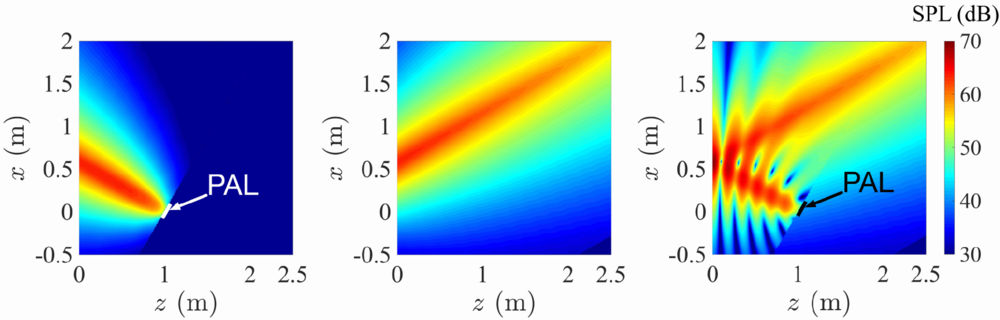
\includegraphics[width = 0.95\textwidth]{Figures/pending/ComputePalReflectionTruncated_3in1_D1B_resize.png}
    \begin{subfigure}{0.32\textwidth}
        \centering
        % \includegraphics[width = \textwidth]{E:/Research/Archive/PalReflection1907/matlab/matlab/reflection/fig/ComputePalReflectionTruncated_Ultra60000_LocSurface1m_Orignal_211013A.pdf}
        \includegraphics[width = \textwidth]{fig/ComputePalReflectionTruncated_Ultra60000_LocSurface1m_Orignal_211013A.pdf}
    \end{subfigure}
    \begin{subfigure}{0.32\textwidth}
        \centering
        % \includegraphics[width = \textwidth]{E:/Research/Archive/PalReflection1907/matlab/matlab/reflection/fig/ComputePalReflectionTruncated_Ultra60000_LocSurface1m_Image_211013B.pdf}
        \includegraphics[width = \textwidth]{fig/ComputePalReflectionTruncated_Ultra60000_LocSurface1m_Image_211013B.pdf}
    \end{subfigure}
    \begin{subfigure}{0.32\textwidth}
        \centering
        % \includegraphics[width = \textwidth]{E:/Research/Archive/PalReflection1907/matlab/matlab/reflection/fig/ComputePalReflectionTruncated_Ultra60000_LocSurface1m_Total_211013C.pdf}
        \includegraphics[width = \textwidth]{fig/ComputePalReflectionTruncated_Ultra60000_LocSurface1m_Total_211013C.pdf}
    \end{subfigure}
    \caption{Audio \revA{SPL (dB re 20 $\mu$Pa)} at 1 kHz generated by: (a) the original PAL in free field; (b) the image PAL with respect to the reflecting surface; and (c) the PAL near a rigid reflecting surface.}
    \label{fig:reflection0}
\end{figure}

For comparison with traditional sources, the incident, reflected, and total sound radiated by an audio piston source and a traditional directional sound source are calculated and shown in Fig.~\ref{fig:reflection:traditional_source} at 1 kHz. 
The piston source is the same size as the PAL and mounted on an infinitely large baffle, so the sound radiates only in the forward direction. 
The directional source is a compact end-fire array consisting of five point monopoles with an interval of 0.045 m as described in \cite{Tu2016RobustnessCompactEndfire}. 
By comparing Figs.~\ref{fig:reflection0} and \ref{fig:reflection:traditional_source}, it can be found that the reflection for the audio sound generated by the PAL is much stronger than that generated by the other two traditional audio sound sources.

\begin{figure}[!htb]
    \centering
    % \includegraphics[width = 0.95\textwidth]{Figures/pending/CircPiston_EndfireArray.pdf}
    % \\
    \begin{subfigure}{0.32\textwidth}
        \centering
        % \includegraphics[width = \textwidth]{E:/Research/Archive/PalReflection1907/matlab/matlab/piston/fig/ComputeCircPistonReflection_1000Hz_Incident_211013D.pdf}
        \includegraphics[width = \textwidth]{fig/ComputeCircPistonReflection_1000Hz_Incident_211013D.pdf}
    \end{subfigure}
    \begin{subfigure}{0.32\textwidth}
        \centering
        % \includegraphics[width = \textwidth]{E:/Research/Archive/PalReflection1907/matlab/matlab/piston/fig/ComputeCircPistonReflection_1000Hz_Reflected_211013E.pdf}
        \includegraphics[width = \textwidth]{fig/ComputeCircPistonReflection_1000Hz_Reflected_211013E.pdf}
    \end{subfigure}
    \begin{subfigure}{0.32\textwidth}
        \centering
        % \includegraphics[width = \textwidth]{E:/Research/Archive/PalReflection1907/matlab/matlab/piston/fig/ComputeCircPistonReflection_1000Hz_Total_211013F.pdf}
        \includegraphics[width = \textwidth]{fig/ComputeCircPistonReflection_1000Hz_Total_211013F.pdf}
    \end{subfigure}
        \\
    \begin{subfigure}{0.32\textwidth}
        \centering
        % \includegraphics[width = \textwidth]{E:/Research/Archive/PalReflection1907/matlab/matlab/endfire/fig/ComputeEndfireReflection_1000Hz_Incident_211013G.pdf}
        \includegraphics[width = \textwidth]{fig/ComputeEndfireReflection_1000Hz_Incident_211013G.pdf}
    \end{subfigure}
    \begin{subfigure}{0.32\textwidth}
        \centering
        % \includegraphics[width = \textwidth]{E:/Research/Archive/PalReflection1907/matlab/matlab/endfire/fig/ComputeEndfireReflection_1000Hz_Reflected_211013H.pdf}
        \includegraphics[width = \textwidth]{fig/ComputeEndfireReflection_1000Hz_Reflected_211013H.pdf}
    \end{subfigure}
    \begin{subfigure}{0.32\textwidth}
        \centering
        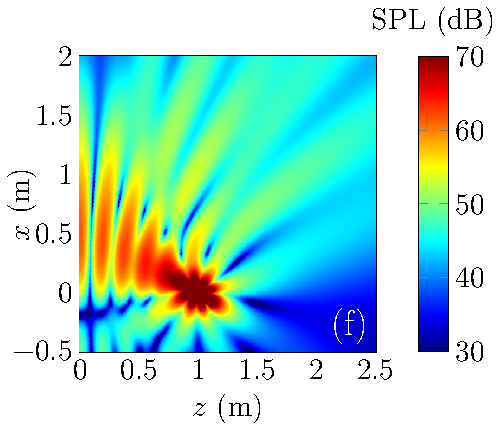
\includegraphics[width = \textwidth]{fig/ComputeEndfireReflection_1000Hz_Total_211013I.pdf}
    \end{subfigure}
    \caption{Audio \revA{SPL (dB re 20 $\mu$Pa)} at 1 kHz where (a), (b), and (c) are the incident, reflected, and total sound radiated by a piston source, respectively, and (d), (c), and (f) are the incident, reflected, and total sound radiated by a 5-channel end-fire array, respectively.}
    \label{fig:reflection:traditional_source}
\end{figure}

The mechanism of the reflected audio sound generated by the PAL is different from that generated by traditional audio sources. 
It can be explained by analyzing the four components in Eq.~(\ref{eq:reflection_component}) for the PAL and the calculated sound fields are shown in Fig.~\ref{fig:reflection:components} using the same parameters in Fig.~\ref{fig:reflection0}. 
The total sound pressure (shown in Fig.~\ref{fig:reflection0}(c)) is the superposition of the audio sound generated by the incident ultrasound ($p\subt{inc,+}$, shown in Fig.~\ref{fig:reflection:components}(a)) and its reflection ($p\subt{inc,-}$, shown in Fig.~\ref{fig:reflection:components}(b)), 
and the audio sound generated by the reflected ultrasound ($p\subt{refl,+}$, shown in Fig.~\ref{fig:reflection:components}(c)) and its reflection ($p\subt{refl,-}$, shown in Fig.~\ref{fig:reflection:components}(d)). 
The audio sound generated by the original PAL (shown in Fig.~\ref{fig:reflection0}(a)) is the superposition of $p\subt{inc,+}$ and $p\subt{refl,-}$, and the one generated by the image PAL (shown in Fig.~\ref{fig:reflection0}(b)) is the superposition of $p\subt{inc,-}$ and $p\subt{refl,+}$. 
It can be found the audio sound generated by the reflected ultrasound ($p\subt{refl,+}$) is the dominant contributor to the directivity of the reflected audio sound of the PAL. 
\begin{figure}[!htb]
    \centering
    % \includegraphics[width = 0.7\textwidth]{Figures/pending/ComputePaaReflectionComponents_All.pdf}
    % \\
    \begin{subfigure}{0.35\textwidth}
        \centering
        % \includegraphics[width = \textwidth]{E:/Research/Archive/PalReflection1907/matlab/matlab/reflection/fig/ComputePalReflectionTruncated_Ultra60000Hz_ByIncidentUltra_211013J.pdf}
        \includegraphics[width = \textwidth]{fig/ComputePalReflectionTruncated_Ultra60000Hz_ByIncidentUltra_211013J.pdf}
    \end{subfigure}
    \begin{subfigure}{0.35\textwidth}
        \centering
        % \includegraphics[width = \textwidth]{E:/Research/Archive/PalReflection1907/matlab/matlab/reflection/fig/ComputePalReflectionTruncated_Ultra60000Hz_ByIncidentUltraReflection_211013K.pdf}
        \includegraphics[width = \textwidth]{fig/ComputePalReflectionTruncated_Ultra60000Hz_ByIncidentUltraReflection_211013K.pdf}
    \end{subfigure}
    \\
    \begin{subfigure}{0.35\textwidth}
        \centering
        % \includegraphics[width = \textwidth]{E:/Research/Archive/PalReflection1907/matlab/matlab/reflection/fig/ComputePalReflectionTruncated_Ultra60000Hz_ByReflectedUltra_211013L.pdf}
        \includegraphics[width = \textwidth]{fig/ComputePalReflectionTruncated_Ultra60000Hz_ByReflectedUltra_211013L.pdf}
    \end{subfigure}
    \begin{subfigure}{0.35\textwidth}
        \centering
        % \includegraphics[width = \textwidth]{E:/Research/Archive/PalReflection1907/matlab/matlab/reflection/fig/ComputePalReflectionTruncated_Ultra60000Hz_ByReflectedUltraReflection_211013M.pdf}
        \includegraphics[width = \textwidth]{fig/ComputePalReflectionTruncated_Ultra60000Hz_ByReflectedUltraReflection_211013M.pdf}
    \end{subfigure}
    \caption{Audio \revA{SPL (dB re 20 $\mu$Pa)} of four components generated by the PAL at 30$^\circ$ incidence near a rigid reflecting surface with a distance of 1 m at 1 kHz: (a) and (b) the audio sound generated by the incident ultrasound and its reflection, respectively; (c) and (d) the audio sound generated by the reflected ultrasound and its reflection, respectively.}
    \label{fig:reflection:components}
\end{figure}
The amplitude of the audio sound generated by reflected sound is affected by the distance between the PAL and the reflecting surface ($D$). 
Figure~\ref{fig:reflection:vary_distance} shows the audio sound field generated by the PAL at $30^\circ$ incidence with reflection surface at $D = \SI{2}{m}$ and 4 m. 
Compared with Fig.~\ref{fig:reflection0}, the amplitude of the audio sound generated by the reflected sound becomes small as $D$ increases. 
This is because the amplitude of the reflected ultrasound becomes smaller when the PAL moves farther away from the reflecting surface, especially when the distance is larger than the effective absorption length (2.17 m in this case).

\begin{figure}[!htb]
    \centering
    % \includegraphics[width = 0.95\textwidth]{Figures/pending/vary_distance.pdf}
    % \\
    \begin{subfigure}{0.32\textwidth}
        \centering
        % \includegraphics[width = \textwidth]{E:/Research/Archive/PalReflection1907/matlab/matlab/reflection/fig/ComputePalReflectionTruncated_Ultra60000_LocSurface2m_Orignal_211013N.pdf}
        \includegraphics[width = \textwidth]{fig/ComputePalReflectionTruncated_Ultra60000_LocSurface2m_Orignal_211013N.pdf}
    \end{subfigure}
    \begin{subfigure}{0.32\textwidth}
        \centering
        % \includegraphics[width = \textwidth]{E:/Research/Archive/PalReflection1907/matlab/matlab/reflection/fig/ComputePalReflectionTruncated_Ultra60000_LocSurface2m_Image_211013O.pdf}
        \includegraphics[width = \textwidth]{fig/ComputePalReflectionTruncated_Ultra60000_LocSurface2m_Image_211013O.pdf}
    \end{subfigure}
    \begin{subfigure}{0.32\textwidth}
        \centering
        % \includegraphics[width = \textwidth]{E:/Research/Archive/PalReflection1907/matlab/matlab/reflection/fig/ComputePalReflectionTruncated_Ultra60000_LocSurface2m_Total_211013P.pdf}
        \includegraphics[width = \textwidth]{fig/ComputePalReflectionTruncated_Ultra60000_LocSurface2m_Total_211013P.pdf}
    \end{subfigure}
    \\
    \begin{subfigure}{0.32\textwidth}
        \centering
        % \includegraphics[width = \textwidth]{E:/Research/Archive/PalReflection1907/matlab/matlab/reflection/fig/ComputePalReflectionTruncated_Ultra60000_LocSurface4m_Orignal_211013Q.pdf}
        \includegraphics[width = \textwidth]{fig/ComputePalReflectionTruncated_Ultra60000_LocSurface4m_Orignal_211013Q.pdf}
    \end{subfigure}
    \begin{subfigure}{0.32\textwidth}
        \centering
        % \includegraphics[width = \textwidth]{E:/Research/Archive/PalReflection1907/matlab/matlab/reflection/fig/ComputePalReflectionTruncated_Ultra60000_LocSurface4m_Image_211013R.pdf}
        \includegraphics[width = \textwidth]{fig/ComputePalReflectionTruncated_Ultra60000_LocSurface4m_Image_211013R.pdf}
    \end{subfigure}
    \begin{subfigure}{0.32\textwidth}
        \centering
        % \includegraphics[width = \textwidth]{E:/Research/Archive/PalReflection1907/matlab/matlab/reflection/fig/ComputePalReflectionTruncated_Ultra60000_LocSurface4m_Total_211013S.pdf}
        \includegraphics[width = \textwidth]{fig/ComputePalReflectionTruncated_Ultra60000_LocSurface4m_Total_211013S.pdf}
    \end{subfigure}
    \caption{Audio \revA{SPL (dB re 20 $\mu$Pa)} generated by the original PAL and the image PAL, and the total sound fields with different distance between the PAL and the reflecting surface. (a-c) the distance is 2 m, and (d-f) the distance is 4 m.}
    \label{fig:reflection:vary_distance}
\end{figure}


\begin{figure}[!htb]
    \centering
    % \includegraphics[width = 0.95\textwidth]{Figures/pending/vary_soundAsborpCoeff.pdf}
    \begin{subfigure}{0.32\textwidth}
        \centering
        % \includegraphics[width = \textwidth]{E:/Research/Archive/PalReflection1907/matlab/matlab/reflection/fig/ComputePalReflectionTruncated_Ultra60000_LocSurface1m_Absorp50_Orignal_211013T.pdf}
        \includegraphics[width = \textwidth]{fig/ComputePalReflectionTruncated_Ultra60000_LocSurface1m_Absorp50_Orignal_211013T.pdf}
    \end{subfigure}
    \begin{subfigure}{0.32\textwidth}
        \centering
        % \includegraphics[width = \textwidth]{E:/Research/Archive/PalReflection1907/matlab/matlab/reflection/fig/ComputePalReflectionTruncated_Ultra60000_LocSurface1m_Absorp50_Image_211013U.pdf}
        \includegraphics[width = \textwidth]{fig/ComputePalReflectionTruncated_Ultra60000_LocSurface1m_Absorp50_Image_211013U.pdf}
    \end{subfigure}
    \begin{subfigure}{0.32\textwidth}
        \centering
        % \includegraphics[width = \textwidth]{E:/Research/Archive/PalReflection1907/matlab/matlab/reflection/fig/ComputePalReflectionTruncated_Ultra60000_LocSurface1m_Absorp50_Total_211013V.pdf}
        \includegraphics[width = \textwidth]{fig/ComputePalReflectionTruncated_Ultra60000_LocSurface1m_Absorp50_Total_211013V.pdf}
    \end{subfigure}
    \\
    \begin{subfigure}{0.32\textwidth}
        \centering
        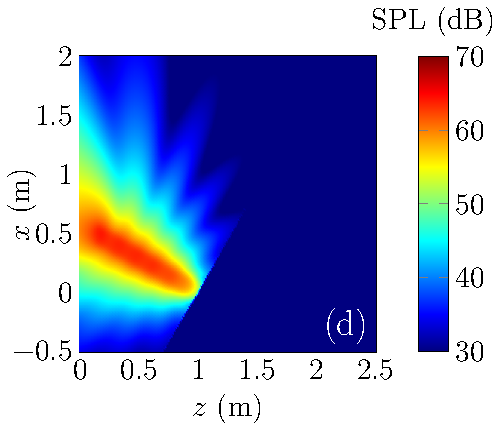
\includegraphics[width = \textwidth]{fig/ComputePalReflectionTruncated_Ultra60000_LocSurface1m_Absorp90_Orignal_211013W.pdf}
    \end{subfigure}
    \begin{subfigure}{0.32\textwidth}
        \centering
        % \includegraphics[width = \textwidth]{E:/Research/Archive/PalReflection1907/matlab/matlab/reflection/fig/ComputePalReflectionTruncated_Ultra60000_LocSurface1m_Absorp90_Image_211013X.pdf}
        \includegraphics[width = \textwidth]{fig/ComputePalReflectionTruncated_Ultra60000_LocSurface1m_Absorp90_Image_211013X.pdf}
    \end{subfigure}
    \begin{subfigure}{0.32\textwidth}
        \centering
        % \includegraphics[width = \textwidth]{E:/Research/Archive/PalReflection1907/matlab/matlab/reflection/fig/ComputePalReflectionTruncated_Ultra60000_LocSurface1m_Absorp90_Total_211013Y.pdf}
        \includegraphics[width = \textwidth]{fig/ComputePalReflectionTruncated_Ultra60000_LocSurface1m_Absorp90_Total_211013Y.pdf}
    \end{subfigure}
    \caption{Audio \revA{SPL (dB re 20 $\mu$Pa)} generated by the original PAL and its image, and the total sound field with different sound absorption coefficient of the reflecting surface. (a-c) are for ultrasound absorption coefficient of 0.5; and (d-f) are for ultrasound absorption coefficient of 0.9.}
    \label{fig:reflection:vary_sound_absorp_coef}
\end{figure}

\begin{figure}[!htb]
    \centering
    % \includegraphics[width = 0.95\textwidth]{Figures/pending/vary_CarrierFreq.pdf}
    % \\
    \begin{subfigure}{0.32\textwidth}
        \centering
        % \includegraphics[width = \textwidth]{E:/Research/Archive/PalReflection1907/matlab/matlab/reflection/fig/ComputePalReflectionTruncated_Ultra100000_LocSurface1m_Absorp0_Orignal_211013Z.pdf}
        \includegraphics[width = \textwidth]{fig/ComputePalReflectionTruncated_Ultra100000_LocSurface1m_Absorp0_Orignal_211013Z.pdf}
    \end{subfigure}
    \begin{subfigure}{0.32\textwidth}
        \centering
        % \includegraphics[width = \textwidth]{E:/Research/Archive/PalReflection1907/matlab/matlab/reflection/fig/ComputePalReflectionTruncated_Ultra100000_LocSurface1m_Absorp0_Image_211013Aa.pdf}
        \includegraphics[width = \textwidth]{fig/ComputePalReflectionTruncated_Ultra100000_LocSurface1m_Absorp0_Image_211013Aa.pdf}
    \end{subfigure}
    \begin{subfigure}{0.32\textwidth}
        \centering
        % \includegraphics[width = \textwidth]{E:/Research/Archive/PalReflection1907/matlab/matlab/reflection/fig/ComputePalReflectionTruncated_Ultra100000_LocSurface1m_Absorp0_Total_211013Ab.pdf}
        \includegraphics[width = \textwidth]{fig/ComputePalReflectionTruncated_Ultra100000_LocSurface1m_Absorp0_Total_211013Ab.pdf}
    \end{subfigure}
    \begin{subfigure}{0.32\textwidth}
        \centering
        % \includegraphics[width = \textwidth]{E:/Research/Archive/PalReflection1907/matlab/matlab/reflection/fig/ComputePalReflectionTruncated_Ultra200000_LocSurface1m_Absorp0_Orignal_211013Ac.pdf}
        \includegraphics[width = \textwidth]{fig/ComputePalReflectionTruncated_Ultra200000_LocSurface1m_Absorp0_Orignal_211013Ac.pdf}
    \end{subfigure}
    \begin{subfigure}{0.32\textwidth}
        \centering
        % \includegraphics[width = \textwidth]{E:/Research/Archive/PalReflection1907/matlab/matlab/reflection/fig/ComputePalReflectionTruncated_Ultra200000_LocSurface1m_Absorp0_Image_211013Ad.pdf}
        \includegraphics[width = \textwidth]{fig/ComputePalReflectionTruncated_Ultra200000_LocSurface1m_Absorp0_Image_211013Ad.pdf}
    \end{subfigure}
    \begin{subfigure}{0.32\textwidth}
        \centering
        % \includegraphics[width = \textwidth]{E:/Research/Archive/PalReflection1907/matlab/matlab/reflection/fig/ComputePalReflectionTruncated_Ultra200000_LocSurface1m_Absorp0_Total_211013Ae.pdf}
        \includegraphics[width = \textwidth]{fig/ComputePalReflectionTruncated_Ultra200000_LocSurface1m_Absorp0_Total_211013Ae.pdf}
    \end{subfigure}
    \\
    \caption{Audio \revA{SPL (dB re 20 $\mu$Pa)} generated by the PAL, its image and the total sound field \revA{at $30^\circ$} incidence near a rigid reflecting surface with $D = \SI{1 }{m}$. (a-c) are for the ultrasound frequencies of 100 kHz and 101 kHz, (d-f) are for the ultrasound frequencies of 200 kHz and 201 kHz.}
    \label{fig:reflection:ultrasound_freq}
\end{figure}
In some applications, reflecting surfaces such as thin carpets can be highly absorbent for the ultrasound but less absorbent for audio sound. 
Figure~\ref{fig:reflection:vary_sound_absorp_coef} shows the audio sound generated by the original PAL and its image, 
as well as the total sound fields when the sound absorption coefficient of the reflecting surface is 0.5 and 0.9 for ultrasound $(1 - \abs{\scrR(\omega_1)\scrR^*(\omega_2)})$, 
and 0 for audio sound. Because the reflected ultrasound is small with a large sound absorption coefficient, the total sound pressure mainly consists of the audio sound generated by the incident ultrasound. The directivity of the reflected audio beams becomes worse for a larger ultrasound absorption coefficient of the reflecting surface.

Sound absorption in air is different at different frequencies, especially at high frequencies. 
Figure~\ref{fig:reflection:ultrasound_freq} shows the audio sound of PAL at $30^\circ$ incidence with reflection when $D =\SI{1}{ m}$. 
The ultrasound frequencies are 100 kHz and 101 kHz, or 200 kHz and 201 kHz. 
The absorption coefficients at 100 kHz (101 kHz) and 200 kHz (201 kHz) in air are 0.38 Np/m and 0.95 Np/m, respectively. 
The effective absorption lengths at 100 kHz (101 kHz) and 200 kHz (201 kHz) in free field are 1.32 m and 0.53 m, respectively. 
It can be found by comparing Fig.~\ref{fig:reflection:ultrasound_freq} with Fig.~\ref{fig:reflection0} that the amplitude of reflected audio beams decreases and the directivity deteriorates as the ultrasound frequency increases. 
All of aforementioned analyses demonstrate that the reflection of audio sound generated by a PAL differ from the traditional directional source because the properties of ultrasound should be taken into account.


\subsection{Experiments}
Experiments were conducted in a hemi-anechoic room with dimensions of $\SI{7.20}{m} \times\SI{ 5.19}{ m} \times\SI{ 6.77 }{m}$ (height). 
A sketch and photos of the experimental setup are shown in Figs.~\ref{fig:reflection:exp:setup} and \ref{fig:reflection:exp:photo}, respectively. The sound field generated by a PAL, a traditional omnidirectional loudspeaker (point monopole), and a horn loudspeaker (directional source) with and without a cotton sheet on ground were measured at 1 kHz. 
% The preliminary test shows that the cotton sheet used in experiments has a high absorption coefficient for ultrasonic sound (more than 0.8) and 
% a low absorption coefficient for audio sound at 1 kHz (about 0.05).

\begin{figure}[!htb]
    \centering
    \includegraphics[width = 0.85\textwidth]{Figures/pending/ExperimentSetup.pdf}
    \caption{Sketch of the experimental setup when a PAL radiates toward ground with and without a cotton sheet.}
    \label{fig:reflection:exp:setup}
\end{figure}

\begin{figure}[!htb]
    \centering
    \includegraphics[width = 0.95\textwidth]{Figures/pending/ExperimentSetup_v2.jpg}
    \caption{\revA{Photos of the experimental setups when different loudspeakers radiate toward the ground without the cotton sheet: (a) the PAL, (b) the traditional omnidirectional loudspeaker, and (c) the horn loudspeaker, and with the cotton sheet: (d) the PAL, (e) the traditional omnidirectional loudspeaker, and (f) the horn loudspeaker.}}
    \label{fig:reflection:exp:photo}
\end{figure}

Figure~\ref{fig:reflection:exp:setup} shows a sketch of the experimental setup when the PAL radiates toward ground. The sound field was measured at many points distributed on a vertical plane across the center of the testing loudspeaker. The length and the height of the measurement plane are 3 m and 2.5 m, respectively. A custom made 60-channel microphone array with the microphone spacing of 5 cm was used to measure the sound pressure. The spacing between measurement points in the vertical direction is 5 cm when the microphone array is close to the loudspeaker, and 10 cm in the other areas. All measurement microphones were Brüel \& Kjær Type 4957 microphones and they were calibrated by a Brüel \& Kjær Type 4231 calibrator. The sound pressure was sampled with a Brüel \& Kjær PULSE system (the analyzer 3053-B-120 with the input panel UA-2107-120) and the fast Fourier transform (FFT) analyzer in PULSE LabShop was used to obtain the FFT spectrum. The frequency span was set to 6.4 kHz with 6400 lines and the averaging type is linear with 66.67\% overlap and 30 s duration.

The PAL, point monopole sound source, and traditional directional source used in the experiments are a Holosonics Audio Spotlight AS-24i with the surface size of $\SI{60}{cm} \times\SI{ 60}{cm}$, a Genelec 8010A traditional voice coil loudspeaker, and a Daichi dome horn loudspeaker with a $\SI{24}{cm}\times\SI{ 8 }{cm}$ rectangular opening, respectively. 
The carrier frequency of the PAL is 64 kHz according to measurements with a Brüel \& Kjær Type 4939 microphone, and the audio frequency in the experiments was set to 1 kHz. 
The radiating surface of the PAL is covered by a 6 mm thick perspex panel with a hole of radius 10 cm at its center to simulate the circular PAL used in simulations, as shown in Fig.~\ref{fig:reflection:exp:photo}(a). 

To ensure the perspex panel is thick enough to block the audio sound generated by the PAL, further experimental results (not presented here) show that the sound pressure levels on the radiation axis of the PAL decrease by more than 30 dB at 1 kHz when the PAL is covered by a same size perspex panel without the hole.
Therefore, a circular piston source was constructed using the 6 mm thick panel with a hole. 
To avoid spurious sound at microphones induced by the intensive ultrasound radiated by the PAL \cite{Ji2019ExperimentalInvestigationParameters}, all the microphones were covered by a piece of small and thin plastic film in the tests.
\revA{The antialiasing filter in the PULSE system also helps reduce the contamination of the ultrasound pressure.}
The experimental results (not presented here) show the insertion loss of this plastic film is more than 35 dB at 64 kHz and less than 0.6 dB at 1 kHz.
The relative humidity and the temperature in the experiments were 68\% and 25.4\celsius, respectively.


% A thin cotton sheet was used in the experiments to simulate a surface with high absorption for ultrasound at 64 kHz but low absorption for audio sound at 1 kHz. The thickness of the sheet is 250 $\mu\rmm$ and the surface density is $\SI{0.12}{kg/m^2}$. 
A thin cotton sheet was used in the experiments. 
The thickness of the sheet is 250 $\mu\rmm$ and the surface density is $\SI{0.12}{kg/m^2}$. 
The size of the cotton sheet is $\SI{2.8}{m}\times \SI{ 4 }{m}$ and placed on the ground so that the projection of the center of the loudspeaker is on the bisector with respect to the narrower side (2.8 m), as shown in Fig.~\ref{fig:reflection:exp:setup}. 
% The sound absorption coefficient of the cotton sheet was measured according to the two-microphone method specified in ISO10534-2 using the Brüel \& Kjær Type 4206 Impedance Tube and the value is 0.05 at 1 kHz \cite{2001ISO1053422001}, so it has little effects on the audio sound generated by the traditional loudspeakers.
\revA{The impedance tube (Brüel \& Kjær Type 4206) was used to measure the absorption coefficient according to the two-microphone method specified in ISO 10523-2 {\cite{2001ISO1053422001}}. 
The result measured at 1 kHz is approximately 0.05 demonstrating that a little  audio sound energy was absorbed by the cotton sheet. So, it has negligible effects on the audio sound generated by the traditional loudspeakers.}

\revA{Figure~{\ref{fig:reflection:exp:results}} shows the measured sound fields at 1 kHz generated by different loudspeakers at $30^\circ$ incidence, 
with and without the cotton sheet on ground.}
Due to operation difficulties, 
the sound fields in the rectangular regions $(\SI{0.85}{m} \leq z \leq \SI{2.5}{m}, \SI{-0.5}{m} \leq x \leq \SI{0.35}{m})$, $(\SI{1}{m}\leq  z \leq \SI{1.2}{m}, \SI{-0.5 }{m} \leq x \leq\SI {0.35 }{m})$, and $(\SI{0.9 }{m} \leq z \leq \SI{1.3 }{m}, \SI{-0.5 }{m} \leq x \leq\SI{ 0.35}{ m}$) were not measured for the 3 configurations, respectively, which are marked as blank regions in the figures.
\begin{figure}[!htb]
    \centering
    \includegraphics[width = 0.95\textwidth]{Figures/pending/AllExperimentalResults-Resize.jpg}
    \caption{Measured \revA{audio SPL (dB re 20 $\mu$Pa)} at 1 kHz generated by different loudspeakers at $30^\circ$ incidence without the cotton sheet for: (a) the PAL, (b) the traditional omnidirectional loudspeaker and (c) a horn loudspeaker, and with the cotton sheet on the ground for: (d) the PAL, (e) the traditional omnidirectional loudspeaker, and (f) a horn loudspeaker.}
    \label{fig:reflection:exp:results}
\end{figure}
It can be seen in Fig.~\ref{fig:reflection:exp:results}(a) that the reflected audio sound is still highly focused on the axis in the reflection direction.
\revA{This agrees with the numerical simulations presented in Fig.~{\ref{fig:reflection0}}(c).}
However, the audio sound drops by up to 6 dB on the reflection axis with the cotton sheet placed on ground, as shown in Fig.~{\ref{fig:reflection:exp:results}}(d). 
\revA{The results are similar to the simulation presented in Fig.~{\ref{fig:reflection:vary_sound_absorp_coef}}(f), where the ultrasound absorption coefficient is assumed to be 0.9.
    It demonstrates the ultrasound reflects a little with respect to the cotton sheet used in experiments and consequently affects the generation of audio sound.
}
However, the reflected sound generated by the traditional loudspeakers are almost the same with and without the cotton sheet. The results indicate that the reflected audio sound generated by the PAL are not only the reflection of audio sound generated by incident ultrasound, and they also contain new audio sound generated by reflected ultrasound, and it is the latter that determines the directivity of the reflected audio sound.


\section{Transmission through a thin partition}
\label{sec:phys_transmission}

It is found in experiments the directivity of audio sound generated by a PAL deteriorates significantly after introducing a thin and homogeneous partition. 
Understanding the insertion loss of the partition for audio sound generated by a PAL is important in applications. 
For example, with the capability of producing quasi-plane waves, PALs can be used to measure the acoustic parameters of materials in situ by measuring the sound pressure on the transmission side of the specimen \cite{Castagnede2008LowFrequencySitu}. 
The sharp directivity of PALs is attractive to mobile phone designers \cite{Ahn2019CriticalStepUsing}. 
However, the size of the effective radiation surface should be as large as possible to generate considerable sound levels. 
A natural way is to install a PAL under the phone screen, so the effects of the thin screen on the generated audio sound need to be known. 
In research, one may need a circular PAL in experiments for verifying the analytical model, but there are only square/rectangular commercial PALs. 
It is shown in Sec.~\ref{sec:transmission_sim} that a circular PAL can be constructed by covering a square one with a 6 mm thick perspex panel.

\revA{The thin partition considered in this section implies that the thickness of the partition is small compared to the audio wavelength and the effective absorption distance of the PAL.}
The transmission of an audio plane wave through a thin partition is well known and the mass law is widely used to predict the insertion loss \cite{Pierce2019AcousticsIntroductionIts}. 
The effects of a thin partition on spherical waves radiated by a point monopole were also studied where the transmission loss and the insertion loss are derived analytically using the plane wave expansion method \cite{Shi2008SoundInsulationInfinite}. 
The transmission of a diffuse incident sound through a partition has also been well studied \cite{Pellicier2007ReviewAnalyticalMethods}. 
However, there is little research reported on the transmission of audio sound generated by a PAL through a thin partition. 
Existing analytical models of PALs consider the sound radiation in free field but pay little attention to its transmission through a partition, which will be resolved in this section.


\subsection{Theory}

A sketch of a PAL radiating sound through a partition is shown in Fig.~\ref{fig:partition}, where the radiation axis of the PAL is perpendicular to the partition surface for simplicity.
The density and the sound speed in air are $\rho_0$ and $c_0$, respectively.
A rectangular coordinate system $Oxyz$ is established with its origin $O$ at the projection of the center of the PAL on the partition surface and the $z$\mbox{-axis} is perpendicular to the surface.
The center of the PAL is at $(0,0,z\subt{P})$ where $z\subt{P} <0$. 
The thickness of the infinitely large partition is assumed to be small enough compared to the audio wavelength and the effective absorption length of the PAL for simplicity. 
The partition is placed at $z=0$ and its area density is denoted by $M$.
\begin{figure}[!htb]
    \centering
    \includegraphics[width=0.6\textwidth]{Figures/PALpartitionv2.jpg}
    \caption{Sketch for a PAL near a thin partition.}
    \label{fig:partition}
\end{figure}
When ultrasound at two different frequencies $f_1$ and $f_2$ ($f_1>f_2$) are generated by the PAL, infinitely many virtual audio sources with the frequency $f\subt{a} = f_1-f_2$ are formed everywhere as long as there exists ultrasound under the quasilinear assumption. 
When the ultrasound is incident on the partition, there are reflected and transmitted ultrasound with respect to the partition and they produce new virtual audio sources on the incident ($z<0$) and transmission ($z>0$) sides, respectively.
The audio sound generated by the ultrasound inside the partition is very small, so they are neglected for simplicity.

The audio sound generated by these three kinds of virtual audio sources, i.e., those generated by incident, reflected , and transmitted ultrasound, all propagate through the partition and there are consequently reflected and transmitted audio sound. 
In this section, only the audio sound on the transmission side ($z>0$) is considered for calculating the insertion loss of the partition.
Based on the above analysis, there are four audio sound components on the transmission side: the transmitted audio sound generated by the incident and reflected ultrasound, the audio sound generated by the transmitted ultrasound and its reflection on the transmission side.

Because the audio sound generated by the reflected ultrasound radiates in the direction which is away from the partition toward the PAL source direction, the transmitted sound of these audio sound is small and can be neglected.
Similarly, the reflection of the audio sound generated by the
transmitted ultrasound can be neglected as well. Therefore,
two audio sound components dominate the sound field on
the transmission side, so the total sound pressure of audio
sound can be expressed approximately as
\begin{equation}
    \Phi\subt{tot}(\vb{r},k\subt{a}) = \Phi\subt{inc}(\vb{r},k\subt{a}) + \Phi\subt{trans}(\vb{r}, k\subt{a})\qc
    z>0
\end{equation}
where $\Phi\subt{inc}(\vb{r},k\subt{a})$ and $\Phi\subt{trans}(\vb{r}, k\subt{a})$ represent the transmitted sound
of the audio sound generated by incident ultrasound and
the audio sound generated by transmitted ultrasound,
respectively.

\subsubsection{Transmission of audio sound generated by incident ultrasound}
The incident ultrasound can be calculated by the
Rayleigh integral as
\begin{equation}
    \Phi\subt{inc}(\vb{r},k_i)
    = -2u_0
    \iint_S 
    g(\vb{r},\vb{r}\subt{s}, k_i + \rmi \alpha_i )
    \dd^2 \bm{\uprho}\subt{s}
    \qc
    z\subt{s} < z <0 
\end{equation}
where the time dependence $\rme^{-\rmi \omega_i t}$  is omitted, 
and the PAL is assumed to be driven by a baffled
piston with the velocity amplitude $u_0$ for both ultrasonic
waves over the surface $S$. The wavenumber $k_i=\omega_i/c_0$,
$i = 1,2$, 
$|\vb{r}-\vb{r}\subt{s}|$ is the distance
between the field point $\vb{r}$ and the source point
$r\subt{s}$ on the PAL surface.

The transmitted sound of the audio sound generated by
incident ultrasound at the field point r on the incident side
can be expressed as
\begin{equation}
    \Phi\subt{inc}(\vb{r},k\subt{a})
    = -
    \int_{z\subt{s}}^0
    \int_{-\infty}^\infty
    \int_{-\infty}^\infty
    q\subt{inc}(\vb{r}\subt{v})
    g(\vb{r},\vb{r}\subt{v}, k\subt{a} +\rmi \alpha\subt{a})
    \dd^3 \vb{r}\subt{v}
    \qc
    z\subt{s} < z < 0
    \label{eq:transmission_audio_potential}
\end{equation}
where the source density function at the virtual source point $\vb{r}\subt{v}$ is
\begin{equation}
    q\subt{inc} (\vb{r}\subt{v})
    =  \frac{\beta \omega\subt{a} \omega_1\omega_2}{\rmi c_0^4}
    \Phi\subt{inc}(\vb{r}\subt{v}, k_1)
    \Phi\subt{inc}^*(\vb{r}\subt{v}, k_2)
    \qc
    z\subt{s} < z\subt{v} <0
\end{equation}
It should be noted that Eq.~(\ref{eq:transmission_audio_potential}) is derived based on the
Westervelt equation, where the Lagrangian density
characterizing the local effects is neglected \cite{Aanonsen1984DistortionHarmonicGeneration, Cervenka2019VersatileComputationalApproach}. Further
simulations 
verify that the error is less than 0.2 dB when the distance
between the field point and the PAL is larger than
0.3 m for the parameters used in this section, which indicates
that the method is sufficiently accurate for the
model investigated.
% find the results in rebuttal letter

The transmitted sound of the audio sound generated
by incident ultrasound can be calculated by using the
plane wave expansion (Sec.~26 in \cite{Brekhovskikh1980WavesLayeredMedia} or Chap.~2 in
\cite{Williams1999FourierAcousticsSound}). 
For a point monopole located at $\vb{r}\subt{m} = (x\subt{m}, y\subt{m},z\subt{m})$ 
with a source strength of $Q\subt{m}$, the transmitted sound at
field point $\vb{r}$ on the transmission side of the partition can
be expressed as \cite{Shi2008SoundInsulationInfinite}
\begin{equation}
    \Phi\subt{trans, m} (\vb{r}) = 
    -\frac{Q\subt{m} }{4\uppi}
    \calK(\vb{r},\vb{r}\subt{m})\qc
    z>0\qc z\subt{m} < 0
\end{equation}
where the Weyl's integral is expressed as, see Eq.~(2.65) in \cite{Williams1999FourierAcousticsSound}
\begin{equation}
    K(\vb{r},\vb{r}\subt{m})
    =
    \frac{\rmi}{2\uppi}
    \int_{-\infty}^\infty
    \int_{-\infty}^\infty
    \frac{\scrT \subt{plane} }{k_{\mathrm{a}, z}} 
    \rme^{\rmi \qty[k_x(x-x\subt{m}) + k_y(y-y\subt{m}) + k_{\mathrm{a},z}|z-z\subt{m}|]}
    \dd k_x \dd k_y
    \label{eq:weyl39f}
\end{equation}
where 
\begin{equation}
    k_{\mathrm{a},z} = \sqrt{(k\subt{a} + \rmi \alpha\subt{a})^2 - k_\rho^2}
    \qc
    k_\rho^2 = k_x^2+k_y^2
\end{equation}
the unit of $\calK(\vb{r},\vb{r}\subt{m})$ is the same as the wavenumber.
$\scrT\subt{plane}$ is the
sound pressure transmission coefficient for the plane wave
with the wavevector $\vb{k}\subt{a} = (k_x,k_y, k_{\mathrm{a},z})$, see Sec.~3.8 in \cite{Pierce2019AcousticsIntroductionIts}.
\begin{equation}
    \scrT\subt{plane}
    = \frac{2\rho_0\omega\subt{a} / k_{\mathrm{a},z}}{2\rho_0\omega\subt{a}/k_{\mathrm{a},z} - \rmi \omega\subt{a} M}
\end{equation}
If the thin partition is porous material, the flow resistance is
taken into account and the sound pressure transmission coefficient
is modified as, see Sec.~3.8 in \cite{Pierce2019AcousticsIntroductionIts}
\begin{equation}
    \scrT\subt{plane}
    = \frac{2\rho_0\omega\subt{a} / k_{\mathrm{a},z}}{2\rho_0\omega\subt{a}/k_{\mathrm{a},z} + \qty[1/R\subt{f} -1/(\rmi \omega\subt{a} M)]^{-1}}
\end{equation}
provided that the material is homogeneous, where $R\subt{f}$ is the
specific flow resistance.

With the above expressions, the transmitted sound of
the audio sound generated by incident ultrasound on the
transmission side in Eq.~(\ref{eq:transmission_audio_potential}) is expressed as
\begin{equation}
    \Phi\subt{inc}(\vb{r},k\subt{a})
    = -\frac{\rmi\rho_0\omega\subt{a} }{4\uppi}
    \int_{z\subt{s}}^0 
    \int_{-\infty}^\infty
    \int_{-\infty}^\infty
    q\subt{inc}(\vb{r}\subt{v})
    \calK(\vb{r},\vb{r}\subt{v})
    \dd x\subt{s} \dd y\subt{s}
    \qc
    z>0
    \label{eq:partition_inc_potential}
\end{equation}
It is worth noting that Eq.~(\ref{eq:weyl39f}) is hard to converge
because the small sound attenuation coefficient at the audio
frequency makes the integrand singular at $k_{\rma, z} = \sqrt{(k\subt{a}+\rmi \alpha\subt{a})^2 - k_\rho^2} \approx 0$ when $k_\rho = k\subt{a}$. By using the variable
substitution and the integral representation for the
Bessel function at order zero 
\begin{equation}
    J_0(x) = \frac{1}{\uppi}\int_0^\uppi \rme^{\rmi x\cos\theta}\dd \theta
\end{equation}
Eq.~(\ref{eq:weyl39f}) can be reduced to
\begin{equation}
    \begin{split}
        \calK(\vb{r},\vb{r}\subt{v}) 
        = 
        & \rmi \int_0^{\uppi/2}\scrT\subt{plane} k\subt{a}^2 J_0(k\subt{a}\rho\subt{v}\cos\gamma)
        \rme^{\rmi \sqrt{(k\subt{a}+\rmi \alpha\subt{a})^2 - k\subt{a}^2 \cos^2\gamma} |z-z\subt{v}|} \\
        & \times \frac{\sin\gamma \cos\gamma }{\sqrt{(k\subt{a}+\rmi \alpha\subt{a})^2-k\subt{a}^2\cos^2\gamma}} \dd \gamma\\
        & + \int_0^{\infty}\scrT\subt{plane} k\subt{a}^2 J_0(k\subt{a}\rho\subt{v}\cosh\gamma)
    \rme^{-\sqrt{k\subt{a}^2 \cosh^2 \gamma - (k\subt{a}+\rmi \alpha\subt{a})^2 }|z-z\subt{v}|} \\
        & \times \frac{\sinh\gamma \cosh\gamma }{\sqrt{k\subt{a}^2 \cosh^2\gamma -(k\subt{a}+\rmi \alpha\subt{a})^2}} \dd \gamma
    \end{split}
\end{equation}
where $\rho\subt{v} = \sqrt{(x-x\subt{v})^2 + (y-y\subt{v})^2}$ is the transverse distance
between the field point and the virtual source point, both integrals
on the right-hand side are numerically calculated by the
\revA{Simpson's 1/3 rule}, and the dummy variable of the
second integral, $\gamma$, is replaced by $\tan\qty[(\gamma+1)\uppi/4]$ to transform
the infinitely large interval into a finite one.

\subsubsection{Audio sound generated by transmitted
ultrasound}
Because it is hard to apply the plane wave expansion
directly on the incident ultrasound, the Gaussian beam
expansion (GBE) method is used in this work to simplify the
Rayleigh integral into a finite summation \cite{Wen1988DiffractionBeamField}. 
Although
the GBE method assumes the paraxial approximation for the
ultrasonic waves, further simulations  without the paraxial approximation using the
parameters in this section verify that the calculation errors for
the audio sound are less than 0.4 dB at the positions on the
transmission side. When the PAL is driven by a circular piston
with the radius of $a$, the Rayleigh integral is given by Eq.~(\ref{eq:piston:gbe}).
\begin{equation}
    p\subt{inc}(\vb{r},k_i) = 
    \sum_{n=1}^N \frac{\rho_0c_0u_0 A_n}{1+\rmi B_nz/R_i}
    \rme^{\frac{-B_n}{1+\rmi B_n z/R_i} \qty(\frac{x^2}{a^2}+\frac{y^2}{a^2}) + \rmi (k_i+\rmi \alpha_i)(z-z\subt{s})}
    \qc
    z\subt{s} < z < 0
\end{equation}

The ultrasound can be expanded into plane waves using
the plane wave expansion method to give
\begin{equation}
    \begin{split}
    \Phi\subt{inc}(\vb{r},k_i)
    = &\frac{u_0a^2}{4\uppi \rmi k_i}
    \sum_{n=1}^N \frac{A_n}{B_n}\\
      &\times\iint_{-\infty}^\infty 
    \exp\qty{- \frac{(k_x^2+k_y^2)a^2}{4B_n} + \rmi \qty[k_x x+k_y y + k_{i,z}(z-z\subt{s})]}
    \dd k_x \dd k_y
    \qc
    z\subt{s}<z<0
    \end{split}
\end{equation}
where $k_{i,z} = \sqrt{k_i^2-k_\rho^2}$. 
Similar to Eq.~(\ref{eq:weyl39f}), the transmitted ultrasound can be obtained as
\begin{equation}
    \Phi\subt{trans}(\vb{r},k_i) = 
    \frac{u_0a^2}{2\rmi k_i}
    \sum_{n=1}^N \frac{A_n}{B_n}
    \int_0^\infty \scrT\subt{plane}J_0(k_\rho\rho)k_\rho
    \exp\qty[-\frac{k_\rho^2 a^2}{4B_n} + \rmi k_{i,z}(z-z\subt{s})]\dd k_\rho
    \qc
    z>0
\end{equation}
where $\scrT\subt{plane}$ is the sound pressure transmission coefficient for a
plane wave with the wavevector $\vb{k}_i = (k_x,k_y,k_{i,z})$,
$\rho=\sqrt{x^2+y^2}$, 
and the integral on the right-hand side is
numerically calculated by the \revA{Simpson's 1/3} rule in this
work.

The audio sound generated by transmitted ultrasound
on the transmission side can be expressed as
\begin{equation}
    \Phi\subt{trans}(\vb{r},k\subt{a})
    =-
    \int_0^\infty \int_{-\infty}^\infty \int_{-\infty}^\infty
    q\subt{trans}(\vb{r}\subt{v})
    g(\vb{r},\vb{r}\subt{v},k\subt{a})
    \dd^3 \vb{r}\subt{v}
    \qc
    z>0
    \label{eq:partition_trans_potential}
\end{equation}
where the source density function of the virtual audio source
at $\vb{r}\subt{v}$ is
\begin{equation}
    q\subt{trans}(\vb{r}\subt{v})
    = 
    -\frac{\rmi \beta \omega\subt{a}}{\rho_0^2c_0^4}
    p\subt{trans}(\vb{r}\subt{v},k_1)
    p\subt{trans}^*(\vb{r}\subt{v},k_2)
    \qc
    z\subt{v}>0
\end{equation}

\subsubsection{Insertion loss of the partition}
The insertion loss (IL) of the partition for audio sound
generated by the PAL is defined as the difference of the sound
pressure level (SPL) at a receiver location $\vb{r}$ on the transmission
side without and with the partition
\begin{equation}
    \rmIL\subt{a}(\vb{r}) = 
    20\log_{10} \qty(\left| \frac{p_0(\vb{r},k\subt{a})}{p\subt{tot}(\vb{r},k\subt{a})}\right|) \qty(\mathrm{dB})\qc
    z>0
    \label{eq:partition:389rfjsdpZ}
\end{equation}
where $\log_{10}$ represents the common logarithm with the base
of 10. 
In Eq.~(\ref{eq:partition:389rfjsdpZ}), $p_0(\vb{r},k\subt{a})$ is the sound pressure at $\vb{r}$ without
the partition and can be obtained by changing the upper
limit of the integral with respect to the coordinate $z\subt{v}$ in Eq.
(\ref{eq:transmission_audio_potential}) from 0 into the positive infinity.

For comparison, the insertion loss of the partition for a
plane wave with the normal incidence ($\rmIL\subt{n}$), for a spherical
wave from a point monopole ($\rmIL\subt{m}$), and for a directional incident
sound from a directional end-fire array source consisting
of five point monopoles used in \cite{Tu2016RobustnessCompactEndfire} ($\rmIL\subt{d}$) are
calculated with following equations.
\begin{equation}
    \rmIL\subt{n} = 20\log_{10}
    \qty(\left| \frac{2\rho_0\omega\subt{a}/k_{\rma,z} - \rmi \omega\subt{a} M}{2\rho_0\omega\subt{a}/k_{\rma, z}}\right|) \qty(\rmdB)
\end{equation}
\begin{equation}
    \rmIL\subt{m}(\vb{r}) = 
    20\log_{10}\qty(\left| \frac{\exp\qty(-\alpha\subt{a} | \vb{r}-\vb{r}\subt{m}| )}{|\vb{r}-\vb{r}\subt{m}| \calK(\vb{r},\vb{r}\subt{m})} \right|)
    \qty(\rmdB)\qc
    z>0
\end{equation}
\begin{equation}
    \rmIL\subt{d}(\vb{r})
    = 20\log_{10}
    \qty(\left| \frac{\sum_{n=1}^5 Q_n |\vb{r} - \vb{r}_n|^{-1} \exp\qty[(-\alpha\subt{a} + \rmi k\subt{a})|\vb{r}-\vb{r}_n|]}{\sum_{n=1}^5 Q_n \calK(\vb{r},\vb{r}_n)}\right|)
\end{equation}
where the location of the point monopole $\vb{r}\subt{m} = (x\subt{m}, y\subt{m}, z\subt{m})$,  and the $n$\mbox{-th} point monopole of the end-fire array at $\vb{r}_n = (x_n,y_n,z_n)$  volume velocity $Q_n$.

\subsection{Simulations and discussions}
\label{sec:transmission_sim}
In the following simulations, a circular piston with a radius of a = 0.1 m is driven with a surface vibration velocity amplitude of 0.12 m/s so that the SPL of both ultrasound is approximately 125 dB at 1 m away on the axis when the PAL is placed in the free field.
\revA{The lower ultrasound frequency is set as $f_2 = \SI{60}{kHz}$.}
The ultrasound attenuation coefficient in air is 0.228 Np/m, which is calculated according to ISO 9613-1 at 20\celsius, with a relative humidity of 50\% at standard atmospheric pressure \cite{1993ISO961311993}. 
The Rayleigh distance at 60 kHz is 5.5 m and the absorption length is 2.17 m. 
Two kinds of materials are used as the thin partition in the simulations. The first one is aluminum foil with a thickness of \revA{50\,$\mu$m} and a bulk density of $\SI{2.7 e3 }{kg/m^3}$. 
The second one is a polyester fiber blanket with a thickness of 1 mm, a bulk density of $\SI{20}{kg/m^3}$, and a flow resistivity of $\SI{2e3}{Pa\cdot s/m^2}$ (Table 1 in \cite{Garai2005SimpleEmpiricalModel}). 

In the calculation, the infinitely large integral domain of the integral in Eqs.~(\ref{eq:transmission_audio_potential}) and (\ref{eq:partition_trans_potential}) needs to be reduced to a specific region covering the major energy of ultrasound beams, so the integral domain is reduced to a cylindrical column centered in the axis of the PAL with a radius of 3 m (30 times the PAL radius). 
The expression for the transmitted audio sound generated by incident ultrasound is shown in Eq.~(\ref{eq:partition_inc_potential}), and contains a fourfold integral which is time-consuming for calculating the off-axis field. 
Because $\calK(\vb{r},\vb{r}\subt{v})$ depends only on the transverse distance ($\rho\subt{v}$) and longitudinal distance ($\abs{z - z\subt{v}}$) between the two points, it can be pre-calculated at every transverse and longitudinal distance pairs and then substituted into Eq.~(\ref{eq:partition_inc_potential}) to simplify the integral into a threefold one if the frequency and the thickness of the partition are specified.

Figure~\ref{fig:partition_sim_50mum} compares the audio sound radiated by a PAL, a point monopole and a traditional directional source (5-channel end-fire array \cite{Tu2016RobustnessCompactEndfire}) at $f\subt{a} = \SI{1}{kHz}$ with and without the aluminum partition. 
The source is located at $z\subt{s} = \SI{-1}{ m}$. 
Figures~\ref{fig:partition_sim_50mum}(a), (b), and (c) show the original sound fields of the sources without the partition, while Figs.~\ref{fig:partition_sim_50mum}(d), (e), and (f) show the total sound fields of the sources with the partition where the sound fields on the incident side are not plotted to focus on the sound transmission. 
Figures~\ref{fig:partition_sim_50mum}(a) and (d) are for the PAL, Figs.~\ref{fig:partition_sim_50mum}(b) and (e) are for the point monopole, and Figs.~\ref{fig:partition_sim_50mum}(c) and (f) are for the end-fire array. 
It can be {seen} that the pattern of the sound field generated by a PAL changes significantly behind the partition. 
The audio sound becomes less focused on the radiation axis, showing a deteriorated directivity. 
However, the pattern of sound fields radiated by a point monopole or an end-fire array only change slightly behind the partition. 
The reason is that the directional audio sound radiated by the PAL is generated by ultrasound which are almost blocked by the partition, while the aluminum foil is almost transparent for audio sound radiated by traditional sound sources.

\begin{figure}[!htb]
    \centering
    % \includegraphics[width = 0.95\textwidth]{Figures/pending/厚度50微米_zPal1m_190919C_200605.jpeg}
    \includegraphics[width = 0.95\textwidth]{Figures/pending/thick50_zPal1m_190919C_200605.jpg}
    \caption{Audio \revA{SPL (dB re 20 $\mu$Pa)} at $f_{\mathrm{a}} = \SI{1}{kHz}$ with a ${50}\,\mu{\rmm}$ thick aluminum partition and a source at $z_{\mathrm{s}} = \SI{-1}{m}$ without the partition for the: (a) PAL, (b) point monopole, (c) end-fire array, and with the partition for the: (d) PAL, (e) point monopole, (f) end-fire array. 
    \revA{The lower ultrasound frequency $f_2 = \SI{60}{kHz}$.}}
    \label{fig:partition_sim_50mum}
\end{figure}

Figure~\ref{fig:partition_sim_50mum_aluminum} shows the IL along the radiation axis ($x = 0$) on the transmission side ($z > 0$) with different kinds of sources. 
The IL for the ultrasound is about 35.7 dB, so the audio sound generated by the transmitted ultrasound decreases by about 71.4 dB (as the magnitude of the sound pressure of audio sound is approximately proportional to the square of the magnitude of the one of ultrasound) and can be neglected. 
The IL for the traditional sources (the plane wave, the point monopole, or the end-fire array) is about 3.2 dB while the IL of the audio sound generated by the PAL behind the partition can be greater than 17 dB. 

\begin{figure}[!htb]
    \centering
    \includegraphics[width = 0.5\textwidth]{Figures/pending/CompareAxisIL_fluid_thick50mum_190929B.jpg}
    \caption{Insertion loss of sound radiated by different sources through an aluminum partition with a thickness of $50\,\mu{\mathrm{m}}$.}
    \label{fig:partition_sim_50mum_aluminum}
\end{figure}

The audio sound generated by the PAL behind the partition consists of the transmitted sound of the audio sound generated by incident ultrasound and the audio sound generated by transmitted ultrasound. 
Since most ultrasound is blocked by the partition, audio sound generated by the transmitted ultrasound are negligible, and the audio sound field behind the partition is dominated by the transmitted sound of the audio sound generated by incident ultrasound. 
Large IL (17 dB) for the PAL instead of the small IL (3.2 dB) for the traditional source is observed. 
The effects of the partition on the transmission of the audio sound generated by a PAL and traditional sources is completely different and the transmission of ultrasound should be taken into account for a PAL.

Figure~\ref{fig:partition_sim_1mm} shows the audio sound radiated by different sources behind a partition made of polyester fiber blanket with a thickness of 1 mm for the sources at $z\subt{s} = \SI{-1 }{m}$. 
For a PAL source, audio sound behind the partition are still focused near the radiation axis which is different from the partition made of aluminum. 
This is because the IL of the polyester fiber blanket is not sufficiently large for the ultrasound and some ultrasound can transmit through the partition to form the directivity of audio sound. 
This is demonstrated in Fig.~\ref{fig:partition_sim_1mm_porous}, where the IL of the blanket at 60 kHz is only about 10 dB. 
Figure~\ref{fig:partition_sim_1mm} also illustrates that almost all the sound transmit through the partition for the traditional sound sources because the ILs are almost 0 as shown in Fig.~\ref{fig:partition_sim_1mm_porous}. 
However, most of the audio sound radiated by a PAL are blocked by the partition and the IL is approximately 15 dB.

\begin{figure}[!htb]
    \centering
    % porous_厚度1mm_zPal1m_190922A_200605
    \includegraphics[width = 0.95\textwidth]{Figures/pending/porous_thick1mm_zPal1m_190922A_200605}
    \caption{Audio \revA{SPL (dB re 20 $\mu$Pa)} at $f\subt{a} = \SI{1}{kHz}$ with a 1 mm thick polyester fibre blanket partition and a source at $z\subt{P}$ = \SI{-1}{m}: (a) for a PAL; (b) for a point monopole; (c) an end-fire array.}
    \label{fig:partition_sim_1mm}
\end{figure}

\begin{figure}[!htb]
    \centering
    \includegraphics[width = 0.5\textwidth]{Figures/pending/CompareAxisIL_porous_thick1mm_190929A.jpg}
    \caption{Insertion loss of sound radiated by different sources through a polyester fiber blanket partition with a thickness of 1 mm.}
    \label{fig:partition_sim_1mm_porous}
\end{figure}

Based on the above findings, the effects of the partition thickness on the amplitude and shape of transmitted audio waves can be discussed. 
For a traditional loudspeaker, the insertion loss of a thin partition generally increases by 6 dB when the thickness or the frequency is doubled in the mass law frequency range, so for a \revA{wideband} audio signal, both the amplitude and shape of the transmitted signal changes; however, for a tonal signal, the audio beam shape behind the partition changes a little as the thickness changes. 
For a PAL, if the transmitted audio sound is mainly generated by the transmitted ultrasonic waves, for example, when the partition thickness is smaller than the ultrasonic wavelength, the insertion loss of the partition increases significantly for the ultrasonic waves as the thickness increases, so the transmitted audio waves becomes smaller and less focused due to the reduced ultrasonic waves. 
If the transmitted audio sound is mainly generated by the audio waves generated by the ultrasonic waves on the source side, for example, when the thickness is larger than the ultrasonic wavelength, the effects of the partition thickness are similar to that for a traditional loudspeaker.

\subsection{Experiments}

The experiments were conducted in a semi-anechoic room with dimensions of $\SI{7.20}{m} \times\SI{ 5.19}{ m}\times \SI{6.77}{ m }$ (height). 
The sketch and photographs of experimental setups are shown in Fig.~\ref{fig:partition_exp}.
The sound fields generated by a PAL, a traditional loudspeaker (point monopole), and a horn loudspeaker (directional source) without and with a partition (a sheet of aluminum foil or a cotton sheet) were measured in the experiments.

\begin{figure}[!htb]
    \centering
    \includegraphics[width = 0.8\textwidth]{Figures/pending/Experiment setup all-Resize.jpg}
    \caption{Sketch of the experimental setups; a photo of (b) a 60-channel microphone array; (c) the PAL and the aluminum foil; (d) the traditional loudspeaker (point monopole) and the aluminum foil; (e) the PAL and the cotton sheet; (f) the horn loudspeaker (traditional directional source) and the cotton sheet.}
    \label{fig:partition_exp}
\end{figure}

The sound field was measured at a rectangular grid with $60 \times 41 = 2460$ points and $60 \times 31 = 1860 $ points in the $xOz$ plane for the cases without and with the partition, respectively. 
In all cases, 60 microphones were located in the x direction from $x = \SI{-1.45}{ m}$ to $x = \SI{1.5 }{m}$ with a spacing of 5 cm and they were measured simultaneously with a custom made 60-channel microphone array shown in Fig.~\ref{fig:partition_exp}(b). 
All measurement microphones were Brüel \& Kjær Type 4957 calibrated by the Brüel \& Kjær 4231 calibrator and the sound pressure at microphones was sampled with a Brüel \& Kjær PULSE system (the analyzer 3053-B-120 with the front panel UA-2107-120). 
The fast Fourier transform (FFT) analyzer in PULSE LabShop was used to obtain the FFT spectrum. 
For the cases without the partition, the microphone array was located at 41 different positions in the $z$ direction from $z = \SI{-1 }{m}$ to $z = \SI{3 }{m}$ with the spacing being 10 cm. 
For the cases with the partition, it was located at 31 positions in the $z$ direction from $z = 0$ to $z = \SI{3 }{m}$ with the same spacing being 10 cm. 
In all the measurements, the height of the center of loudspeakers and the microphones is 1.9 m.

The PAL, the point monopole, and the traditional directional source in the experiments were a Holosonics Audio Spotlight AS-24i with the surface size of $\SI{60 }{cm} \times \SI{ 60}{ cm}$, a Genelec 8010A traditional voice coil loudspeaker, and a Daichi dome horn loudspeaker with a $\SI{24 }{cm} \times\SI{ 8}{ cm}$ rectangular opening, respectively. 
The carrier frequency of the PAL is 64 kHz according to the measurements with a Brüel \& Kjær Type 4939 microphone and the audio frequency in the experiments was set to 1 kHz. 
The radiating surface of the PAL was covered by a 6 mm thick perspex panel with a hole of 10 cm radius at the center to construct a circular piston source as shown in Fig.~\ref{fig:partition_exp}(c). 

Further experimental results (not presented here) show that the SPLs on the radiation axis of the PAL decrease by more than 30 dB at 1 kHz when the PAL is covered by a same size square perspex panel, so the panel can provide sufficient IL for audio sound at 1 kHz, which makes the PAL covered by the panel with a hole a circular piston. 
To avoid the spurious sound at microphones induced by the intensive ultrasound radiated by the PAL \cite{Ji2019ExperimentalInvestigationParameters}, all the microphones are covered by a piece of small and thin plastic film. 
The experimental results  show the insertion loss of this plastic film is more than 30 dB at 64 kHz, which is sufficient for blocking the ultrasonic sound, and less than 0.6 dB at 1 kHz, which is negligible for the audio sound under tests.

Two partitions were used in the experiments: a sheet of 50\,$\mu$m thick aluminum foil with a bulk density of $\SI{2.7 e3} {kg/m^3}$ and a 250 $\mu\rmm$  thick cotton sheet with a surface density of $\SI{0.12}{kg/m^2}$. 
The size of the aluminum foil and the cotton sheet are 3.6 m ($x$ direction) $\times$ 3 m ($y$ direction) and 4 m ($x$ direction) $\times$ 2.9 m ($y$ direction), respectively. 
The center of the loudspeaker is at the same height as that of the aluminum foil or the cotton sheet shown in Figs.~\ref{fig:partition_exp}(c-f). 
The relative humidity and the temperature in the experiments were 68\% and 25.4\celsius, respectively. 

Figure~\ref{fig:partition_exp_results} shows the simulation and experimental results of audio sound fields at 1 kHz generated by the three different sound sources which are at 1.9 m high above ground without partitions. 
The experimental results of sound fields generated by the PAL with and without the partition are generally in accordance with the predicted ones shown in Figs.~\ref{fig:partition_exp_results}(a) and (d). 
It can be found the measured sound field radiated by the PAL is highly focused on the radiation axis as expected. 
Some small fluctuations occur in the $z$ axis direction in experimental results which might be caused by reflections of the ground. 
The measured sound fields generated by traditional loudspeakers shown in Figs.~\ref{fig:partition_exp_results}(b-c) and (e-f) also agree well with the simulation ones. 
Figure~\ref{fig:partition_exp_results}(b) is obtained by using the analytical solution of a point monopole above a rigid ground, and Fig.~\ref{fig:partition_exp_results}(c) is obtained by the boundary element method (BEM) solver of the commercial software Virtual.Lab Acoustics. 
\revA{The mesh size of the horn loudspeaker is set as 1.33 cm which is smaller than 1/10 wavelength at 1 kHz, and the model is shown in Fig.~{\ref{fig:fd:jfsdoif}}.}

\begin{figure}[!htb]
    \centering
    \includegraphics[width = 0.5\textwidth]{fig/horn_20220519233959.jpg}
    \caption{\revA{The model of the horn loudspeaker used in Virtual.Lab Acoustics.}}
    \label{fig:fd:jfsdoif}
\end{figure}

\begin{figure}[!htb]
    \centering
    \includegraphics[width = 0.95\textwidth]{Figures/pending/Comparison of experiment and simulations100.jpg}
    \caption{Audio \revA{SPL (dB re 20 $\mu$Pa)} at 1 kHz with different sound sources at $z = \SI{-1}{ m}$ and $x = 0$ above the ground with a height of 1.9 m in the simulations: (a) the PAL, (b) the traditional loudspeaker, and (c) the horn loudspeaker, and in the experiments: (d) the PAL, (e) the traditional loudspeaker, and (f) the horn loudspeaker.}
    \label{fig:partition_exp_results}
\end{figure}

Figure~\ref{fig:partition_exp_results_all} shows the experimental results of audio sound at 1 kHz generated by the three sound sources above the ground with a sheet of aluminum foil and a cotton sheet. 
The sound fields between the loudspeaker ($z = \SI{-1}{ m}$) and the partition ($z = 0$) were not measured because they are not the focus point of this thesis, and {they are} also difficult to measure in practice. 
The theoretical prediction results corresponding to Figs.~\ref{fig:partition_exp_results_all}(a) and (d) are presented in Figs.~\ref{fig:partition_exp_results_sim}(a) and (b), respectively, where reasonable agreements between predictions and experiments are observed. 
The small error might be caused by the unevenness of the partition surface in the experiments. 
It can be found in Fig.~\ref{fig:partition_exp_results_all} that the effects of the thin partitions on the sound transmission loss are small for both the traditional loudspeaker and the horn loudspeaker, but the SPLs generated by a PAL are significantly decreased by the partitions, and audio sound are less focused on the radiation axis behind the partition because most of the ultrasound are blocked by the partition. 
The experiment results support analyses and conclusions in the simulations. 

\begin{figure}[!htb]
    \centering
    \includegraphics[width = 0.95\textwidth]{Figures/pending/AllExperimentalResults2_resize.jpg}
    \caption{Experimental results of the audio \revA{SPL (dB 20 re $\mu$Pa)} at 1 kHz with different sound sources at $z = \SI{-1 }{m}$ and $x = 0$ above the ground with a height of 1.9 m with a sheet of aluminum foil for: (a) the PAL, (b) the traditional loudspeaker, and (c) the horn loudspeaker, and with a cotton sheet for: (d) the PAL, (e) the traditional loudspeaker, and (f) the horn loudspeaker.}
    \label{fig:partition_exp_results_all}
\end{figure}

\begin{figure}[!htb]
    \centering
    \includegraphics[width = 0.8\textwidth]{Figures/pending/Simulations_for_exp_horizontal_resize.jpg}
    \caption{Theoretical prediction audio \revA{SPL (dB re 20 $\mu$Pa)} corresponding to Figs.~\ref{fig:partition_exp_results_all}(a) and (d), i.e. the sound fields at 1 kHz with the PAL at $z = \SI{-1 }{m}$ and $x = 0$ with (a) a sheet of aluminum foil and (b) a cotton sheet.}
    \label{fig:partition_exp_results_sim}
\end{figure}

\section{Scattering by a rigid sphere}
\label{sec:phys_scat}
It is common in some applications for a human to be inside the audible region, which causes scattering of the sound generated by a PAL \cite{Nakashima2005PrototypeParametricArray, Ye2008GenerationAudibleSound}. 
Both the head and torso account for the scattering effect, but the head is the most important part because the ears are on it and only a few sound are incident on the torso when the highly directional beams are generated by a PAL. 
\revA{Besides, there are absorptions at high audio frequencies due to the skin and the hair {\cite{Katz2000AcousticAbsorptionMeasurement}}.
Therefore, a rigid sphere is used here as a first order approximation of the human head in the physical modelling.
The effects of the rigid sphere on the audio sound 
generated by traditional loudspeakers have been well studied to reveal the effects of the human head {\cite{Zou2008PerformanceAnalysisVirtual}}.}
The effects of a sphere on the audio sound generated by a PAL are however different because the sound originates from the nonlinear interactions of waves. 

Based on the Westervelt equation and the quasilinear approximations, an analytic expression for the sound pressure of the DFW was obtained when primary plane waves interact with a rigid sphere \cite{Abbasov1995SphereScatteringNonlinearly}. 
This work showed that the total sound pressure of the DFW is a combination of nonlinear interactions from the incident primary waves (incident-with-incident) and the scattered primary waves (scattered-with-scattered), as well as the incident and scattered primary waves (incident-with-scattered). 
The solution is inaccurate because higher order spherical harmonics in the Green's function are neglected and the scattered waves do not follow the plane wave assumption. 
Furthermore, the accuracy of the Westervelt equation is not examined and the prediction error is large because the local effects near the sphere and between it and the PAL are significant. 
Although full spherical harmonics were considered in \cite{Silva2013DifferencefrequencyGenerationNonlinear}, the calculation was limited to the far field solution. 
The simulation was conducted for a small sphere with the radius of only 1.0 mm, which was insonified by two intersecting plane waves under the water. 
Therefore, the results and conclusions are likely to be different for a sphere with the size of a human head exposed to audio sound generated by a piston-like PAL in air. 
Besides, no detailed experiment results to support the accuracy of these respective studies have been reported to date.

In this section, a computationally efficient method is developed to calculate the quasilinear solution of the audio sound generated by a PAL based on both the Kuznetsov and Westervelt equations. The ultrasound field generated by a circular piston is obtained first by using a spherical harmonic expansion. The audio field is then considered as the radiation from an infinitely large virtual volume source, with the source density proportional to the product of the ultrasonic pressure. The accuracy of the Westervelt equation is then examined and simulations of scattering by a rigid sphere are conducted. Results are compared to those for a traditional loudspeaker and experimental results are presented to validate these predictions.

\subsection{Theory}
A circular PAL radiating towards a rigid sphere is shown in Fig.~\ref{fig:scat_sketch}. 
Both the PAL and the sphere are assumed to be placed in a free field and the PAL is not baffled. 
The radii of the PAL and the sphere are denoted by $a$ and $r_0$, respectively. 
To achieve maximum scattering effects, the center of the sphere is placed on the radiation axis of the loudspeaker. 
The distance between their centers is denoted by $d$. 
A rectangular coordinate system $(x, y, z)$ is established with its origin, $O$, at the center of the sphere and the negative $z$ axis pointing to the center of the PAL. 
The spherical coordinates $(r, \theta, \varphi)$ and the cylindrical coordinates $(\rho, \varphi, z)$ are established with respect to the rectangular coordinates $(x, y, z)$ for further calculations, where $r, \theta, \varphi$, and $\rho$ are the radial distance, zenith angle, azimuth angle, and polar radial distance, respectively.

\begin{figure}[!htb]
    \centering
    \includegraphics[width = 0.7\textwidth]{Figures/TheoryModel}
    \caption{Sketch of a circular PAL near a sphere.}
    \label{fig:scat_sketch}
\end{figure}
\subsubsection{Ultrasound field}
A rigorous approach to modelling the ultrasound field should include scattering from both the non-baffled PAL and the sphere, as well as the interaction between them. 
It has been demonstrated in \cite{Zhong2020NonparaxialModelAudio} that the ultrasound generated by a non-baffled PAL can be approximated by the one generated by a baffled PAL, because the size of the PAL is large enough when compared to the wavelength of the ultrasound. 
The interaction between a PAL and a sphere is known to generate multiple scattering, however when the separation between them is larger than the ultrasonic wavelength and the dimensions of each component, then this scattering is considered to be insignificant \cite{Gaunaurd1995AcousticScatteringPair}.
It is therefore neglected in this thesis for simplicity and to focus on the scattering effects by the sphere.

The ultrasound pressure at a field point $\vb{r} = (r, \theta, \varphi)$ in the presence of a rigid sphere shown in Fig.~\ref{fig:scat_sketch} is solved using the Rayleigh integral,
\begin{equation}
    \Phi(\vb{r}, k_i) = -2\iint_S u(\bm{\uprho}\subt{s},k_i) G(\vb{r},\vb{r}\subt{s},k_i)\dd^2 \bm{\uprho}\subt{s}\qc
    r\geq r_0\qc i = 1,2
    \label{eq:sphere:w89fsjdp}
\end{equation}
where the variables $\bm{\uprho}\subt{s}  = (\rho\subt{s}, \varphi\subt{s})$ are the polar coordinates for the area element on the PAL surface $S$, 
$ \vb{r}\subt{s} = (\rho\subt{s},\varphi\subt{s},z\subt{s})$ are the cylindrical coordinates, and  $z\subt{s}=-d$.
The Green's function $G(\vb{r},\vb{r}\subt{s},k_i)$ is the velocity potential solution at the field point $\vb{r}$ generated by a point monopole at $\vb{r}\subt{s}$ with the unit volume velocity and wavenumber 
$k_i = \omega_i/c_0+\rmi \alpha_i$, \cite{Lin2004ActiveControlRadiation, Zou2007PreliminaryExperimentalStudy}
\begin{equation}
    G(\vb{r},\vb{r}\subt{s}, k_i)
    = 
    \frac{\rmi k_i}{4\uppi}
    \sum_{n=0}^\infty
    (2n+1)R_n(r,r\subt{s},k_i)
    \sum_{m=-n}^n \frac{(n-m)!}{(n+m)!} P_n^m(\cos\theta)P_n^m(\cos\theta\subt{s})
    \rme^{\rmi m (\varphi-\varphi\subt{s})}
    \label{eq:sphere:398fsjpd}
\end{equation}
\begin{equation}
    R_n(r,r\subt{s},k_i) = 
    \rmj_n(k_i r_<)\rmh_n(k_ir_>) - 
    \frac{\rmj_n'(k_ir_0)}{\rmh_n'(k_ir_0)}
    \rmh_n(k_ir)\rmh_n(k_ir\subt{s})
    \label{eq:fskldjfie}
\end{equation}

By substituting Eq.~(\ref{eq:sphere:398fsjpd}) into Eq.~(\ref{eq:sphere:w89fsjdp}), one obtains
\begin{equation}
    \begin{split}
        \Phi(\vb{r},k_i) = \frac{1}{\rmi k_i} 
        \sum_{n=0}^\infty
        &(2n+1)
        \frac{(n-m)!}{(n+m)!} P_n^m(\cos\theta)
        \qty[\frac{1}{2\uppi} \int_0^{2\uppi} \rme^{\rmi m (\varphi-\varphi\subt{s})} \dd \varphi\subt{s}]\\
        &\times \qty[\int_0^a u_i(\rho\subt{s} )R_n(r,r\subt{s},k_i)P_n^m(\cos\theta\subt{s}) k_i^2 \rho\subt{s}\dd\rho\subt{s}]\qc
        r\geq r_0
    \end{split}
    \label{eq:sphere:w9e8fjspdf219}
\end{equation}
with the following relations
\begin{equation}
    \begin{dcases}
        r\subt{s}^2 = \rho\subt{s}^2 +d^2 \Longrightarrow
        r\subt{s}\dd r\subt{s} = \rho\subt{s} \dd \rho\subt{s}\\
        \cos(\uppi-\theta\subt{s}) = \frac{d}{r\subt{s}}
    \end{dcases}
    \label{eq:sphere:2389fjsdpfj}
\end{equation}
By substituting Eq.~(\ref{eq:sphere:2389fjsdpfj}) into Eq.~(\ref{eq:sphere:w9e8fjspdf219}) and using the fact that the integral with respect to $\varphi\subt{s}$ is non-zero when $m = 0$, and the symmetry relation of the Legendre polynomials [see Eq.~(4.2.8) in \cite{Zhang1996ComputationSpecialFunctions}]
\begin{equation}
    P_n(\cos\theta\subt{s}) = P_n\qty(-\frac{d}{r\subt{s}}) = (-1)^n P_n\qty(\frac{d}{r\subt{s}})
\end{equation}
one obtains
\begin{equation}
    \Phi(\vb{r},k_i) = \frac{1}{\rmi k_i}
    \sum_{n=0}^\infty (-1)^n (2n+1) P_n(\cos\theta)\chi_n(r,k_i)\qc
    r\geq r_0
    \label{eq:sphere:phi2891}
\end{equation}
where the radiation component is 
\begin{equation}
    \chi_n(r,k_i) = \int_d^{\sqrt{d^2+a^2}}
    u_i(\rho\subt{s}) R_n(r,r\subt{s},k_i)
    P_n\qty(\frac{d}{r\subt{s}})k_i^2 r\subt{s}\dd r\subt{s}
\end{equation}
Compared to the Rayleigh integral in Eq.~(\ref{eq:sphere:w89fsjdp}), Eq.~(\ref{eq:sphere:phi2891}) is much more efficient to calculate because the convergence of the series is faster than a double integral and the field coordinates are also independent \cite{Mast2005SimplifiedExpansionsRadiation, Zhong2020SphericalExpansionCalculating} The components of the particle velocity of the ultrasound under the spherical coordinate system is then obtained from Eq.~(\ref{eq:sphere:phi2891}) to give
\begin{equation}
    \begin{dcases}
        v_r(\vb{r},k_i) = \pdv{\Phi(\vb{r},k_i)}{r} = -\rmi \sum_{n=0}^\infty
        (-1)^n (2n+1)
        P_n(\cos\theta)
        \dv{\chi_n(r,k_i)}{(k_ir)}\\
        v_\theta(\vb{r}, k_i) = \frac{1}{r}\pdv{\Phi(\vb{r},k_i)}{\theta} 
        = -\rmi \sum_{n=0}^\infty (-1)^n(2n+1)
        \dv{P_n(\cos\theta)}{\theta}
        \frac{\chi_n(r,k_i)}{k_ir}\\
        v_\varphi(\vb{r},k_i) = \frac{1}{r\sin\theta}\pdv{\Phi(\vb{r},k_i)}{\varphi} = 0
    \end{dcases}
\end{equation}

\subsubsection{Audio sound field}
The velocity potential of audio sound is governed by an inhomogeneous Helmholtz equation given by Eq.~(\ref{eq:quasilinear_eq}) under the quasilinear approximation. 
It can be treated as the superposition of sound produced by infinite number of virtual point sources at $\vb{r}\subt{v}$ with the source density function $q(\vb{r}\subt{v})$. 
Therefore, this equation can be solved by integrating the source density using the Green's function with spherical scattering,
\begin{equation}
    \Phi(\vb{r},k\subt{a})
    = -\iiint_{r\subt{v}\geq r_0}
    q(\vb{r}\subt{v}) G(\vb{r}, \vb{r}\subt{v}, k\subt{a}) 
    \dd^3 \vb{r}\subt{v}
    \qc
    r\geq r_0
    \label{eq:scat_potential_audio}
\end{equation}
For a circular PAL with a radius of a and a axisymmetric vibration velocity profile, the source density is not related to the azimuthal angle, so the triple integral of audio sound Eq.~(\ref{eq:scat_potential_audio}) can be simplified to give
\begin{equation}
    \begin{split}
        \Phi(\vb{r},k\subt{a}) = 
        \frac{1}{\rmi k\subt{a}^2}
        \sum_{n=0}^\infty
        & \qty(n+\frac{1}{2})
        \sum_{m=-n}^n \frac{(n-m)!}{(n+m)!}P_n^m (\cos\theta)
        \qty[\frac{1}{2\uppi}\int_0^{2\uppi} \rme^{\rmi m(\varphi-\varphi\subt{v})}\dd \varphi\subt{v}]\\
        &\times
        \int_{0}^\uppi \int_{r_0}^\infty
        q(\vb{r}\subt{v}) R_n(r,r\subt{v},k\subt{a})P_n^m(\cos\theta\subt{v})
        k\subt{a}^3 r\subt{v}^2 \sin\theta\subt{v}
        \dd r\subt{v} \dd \theta\subt{v}
        \qc
        r\geq r_0
    \end{split}
    \label{eq:scat_potential_audio1}
\end{equation}
Similar to Eq.~(\ref{eq:sphere:w9e8fjspdf219}), the integral with respect to $\varphi\subt{v}$ is non-zero when $m = 0$, and Eq.~(\ref{eq:scat_potential_audio1}) then reduces to
\begin{equation}
    \begin{split}
        \Phi(\vb{r},k\subt{a}) = 
        \frac{1}{\rmi k\subt{a}^2}
        \sum_{n=0}^\infty
        &\qty(n+\frac{1}{2}) P_n(\cos\theta)\\
        &\times
        \int_{0}^\uppi \int_{r_0}^\infty
        q(\vb{r}\subt{v}) R_n(r,r\subt{v},k\subt{a})P_n^m(\cos\theta\subt{v})
        k\subt{a}^3 r\subt{v}^2 \sin\theta\subt{v}
        \dd r\subt{v} \dd \theta\subt{v}
        \qc
        r\geq r_0
    \end{split}
    \label{eq:1130912301201020023103123}
\end{equation}

\subsection{Numerical simulations}
Numerical simulations are conducted here using MATLAB R2020b. 
In the simulations, the center frequency of the ultrasound is set as $f\subt{u} = \SI{64}{kHz}$, which is a common value used in commercial PALs. 
The radii of the PAL and the sphere are both set as 0.1 m. 
The distance between the PAL and the sphere, $d$, is set as 1.0 m. 
The audio sound fields generated by a PAL without the sphere are obtained using the spherical harmonic expansion method in \cite{Zhong2020SphericalExpansionAudio, Zhong2021FieldWesterveltFar}. 
The audio sound fields generated by a traditional loudspeaker with and without the sphere are calculated by setting $ka$ in Eq.~(\ref{eq:sphere:phi2891}) and using the method described in \cite{Zhong2020SphericalExpansionCalculating}, respectively. 
A uniform vibration velocity profile is assumed for all cases and an amplitude of $\SI{0.12}{m/s}$ and $\SI{2 e-4}{m/s}$ are set for the ultrasound generated by the PAL and the audio sound generated by the traditional loudspeaker, respectively.

\subsubsection{The accuracy of the Westervelt equation}
Figure~\ref{fig:scat_result_compare_eq} compares the sound pressure level (SPL) for audio sound generated by a PAL using the Westervelt and Kuznetsov equations at different zenith angles, $\theta$, with a distance of 0.1 m or 1.0 m to the center of the sphere at 500 Hz, 1 kHz, and 2 kHz. 
Figure~\ref{fig:scat_result_compare_eq} shows that the audio SPL calculated with the Kuznetsov equation differs from that  obtained using the Westervelt equation, which is also observed for the case without the sphere \cite{Cervenka2019VersatileComputationalApproach, Zhong2021FieldWesterveltFar}. 
The difference between the SPLs calculated using these two equations is large when the observation point is close to the sphere or the PAL. 
For example, at the angle $\theta = 170^\circ$, when the distance between the field point and the center of the sphere is 0.1 m, the difference of SPLs is 16.5 dB, 2.6 dB, and 0.5 dB, at 500 Hz, 1 kHz, and 2 kHz, respectively. When the distance is 1.0 m, fluctuations can be observed when the zenith angle approaches to $180^\circ$ and they are comparable to the ultrasonic wavelength of 5.4 mm at 64 kHz. 
The reason is that the ultrasonic field is complicated, and the pressure is large near the sphere indicating that the local effects are strong, which cannot be correctly captured by the Westervelt equation. 

\begin{figure}[!htb]
    \centering
    \begin{subfigure}{0.49\textwidth}
        \centering
        % \includegraphics[width = \textwidth]{E:/Research/PalSphere1911/matlab/audio/fig/PalSphereAudio_211205D_TestTheta1D_Compare_r10cm_500Hz_211206G.pdf}
        \includegraphics[width = \textwidth]{fig/PalSphereAudio_211205D_TestTheta1D_Compare_r10cm_500Hz_211206G.pdf}
    \end{subfigure}
    \begin{subfigure}{0.49\textwidth}
        \centering
        % \includegraphics[width = \textwidth]{E:/Research/PalSphere1911/matlab/audio/fig/PalSphereAudio_211205D_TestTheta1D_Compare_r100cm_500Hz_211206D.pdf}
        \includegraphics[width = \textwidth]{fig/PalSphereAudio_211205D_TestTheta1D_Compare_r100cm_500Hz_211206D.pdf}
    \end{subfigure}
    \\
    \begin{subfigure}{0.49\textwidth}
        \centering
        \includegraphics[width = \textwidth]{fig/PalSphereAudio_211205D_TestTheta1D_Compare_r10cm_1000Hz_211206C.pdf}
        % \includegraphics[width = \textwidth]{E:/Research/PalSphere1911/matlab/audio/fig/PalSphereAudio_211205D_TestTheta1D_Compare_r10cm_1000Hz_211206C.pdf}
    \end{subfigure}
    \begin{subfigure}{0.49\textwidth}
        \centering
        \includegraphics[width = \textwidth]{fig/PalSphereAudio_211205D_TestTheta1D_Compare_r100cm_1000Hz_211206E.pdf}
        % \includegraphics[width = \textwidth]{E:/Research/PalSphere1911/matlab/audio/fig/PalSphereAudio_211205D_TestTheta1D_Compare_r100cm_1000Hz_211206E.pdf}
    \end{subfigure}
    \\
    \begin{subfigure}{0.49\textwidth}
        \centering
        \includegraphics[width = \textwidth]{fig/PalSphereAudio_211205D_TestTheta1D_Compare_r10cm_2000Hz_211206B.pdf}
        % \includegraphics[width = \textwidth]{E:/Research/PalSphere1911/matlab/audio/fig/PalSphereAudio_211205D_TestTheta1D_Compare_r10cm_2000Hz_211206B.pdf}
    \end{subfigure}
    \begin{subfigure}{0.49\textwidth}
        \centering
        \includegraphics[width = \textwidth]{fig/PalSphereAudio_211205D_TestTheta1D_Compare_r100cm_2000Hz_211206F.pdf}
        % \includegraphics[width = \textwidth]{E:/Research/PalSphere1911/matlab/audio/fig/PalSphereAudio_211205D_TestTheta1D_Compare_r100cm_2000Hz_211206F.pdf}
    \end{subfigure}
    \caption{Audio \revA{SPL (dB re 20 $\mu$Pa)} at different zenith angles with the distance of $d$ to the center of the sphere generated by a PAL: (a) $d = \SI{0.1 }{m}$ at 500 Hz, (b) $d = \SI{1.0}{ m}$ at 500 Hz, (c) $d = \SI{0.1 }{m}$ at 1 kHz, (d) $d = \SI{1.0 }{m }$ at 1 kHz, (e) $d = \SI{0.1 }{m}$ at 2 kHz, and \revA{(f)} $d = \SI{1.0 }{m }$ at 2 kHz. Solid line, Kuznetsov equation; dashed line, Westervelt equation.}
    \label{fig:scat_result_compare_eq}
\end{figure}

The difference between the SPLs using these two equations becomes smaller as the frequency increases. 
This is because the audio SPL calculated with the Westervelt equation increases by about 12 dB when the audio frequency is doubled, but corresponding changes in the amplitude of the ultrasonic Lagrangian density are relatively small, so its effect on the audio SPL is small at high audio frequencies. 
Therefore, it is concluded that the Kuznetsov equation should be used in the calculation, especially for observation points near the sphere at low frequencies. 
Accordingly, all the simulations that follow are obtained using the Kuznetsov equation.

\begin{figure}[!htb]
    \centering
    \begin{subfigure}{0.49\textwidth}
        \centering
        % \includegraphics[width = \textwidth]{E:/Research/PalSphere1911/matlab/audio/fig/PalSphere_211205D_Test2D_Kuznetsov_2000Hz_211211K.pdf}
        \includegraphics[width = \textwidth]{fig/PalNoSphere_2D_211211E_500Hz_211211F.pdf}
    \end{subfigure}
    \begin{subfigure}{0.49\textwidth}
        \centering
        % \includegraphics[width = \textwidth]{E:/Research/PalSphere1911/matlab/audio/fig/PalSphere_211205D_Test2D_Kuznetsov_500Hz_211211I.pdf}
        \includegraphics[width = \textwidth]{fig/PalSphere_211205D_Test2D_Kuznetsov_500Hz_211211I.pdf}
    \end{subfigure}
    \\
    \begin{subfigure}{0.49\textwidth}
        \centering
        % \includegraphics[width = \textwidth]{E:/Research/PalSphere1911/matlab/audio/fig/PalNoSphere_2D_211211E_1000Hz_211211G}
        \includegraphics[width = \textwidth]{fig/PalNoSphere_2D_211211E_1000Hz_211211G}
    \end{subfigure}
    \begin{subfigure}{0.49\textwidth}
        \centering
        % \includegraphics[width = \textwidth]{E:/Research/PalSphere1911/matlab/audio/fig/PalSphere_211205D_Test2D_Kuznetsov_1000Hz_211211J}
        \includegraphics[width = \textwidth]{fig/PalSphere_211205D_Test2D_Kuznetsov_1000Hz_211211J}
    \end{subfigure}
    \\
    \begin{subfigure}{0.49\textwidth}
        \centering
        % \includegraphics[width = \textwidth]{E:/Research/PalSphere1911/matlab/audio/fig/PalNoSphere_2D_211211E_2000Hz_211211H}
        \includegraphics[width = \textwidth]{fig/PalNoSphere_2D_211211E_2000Hz_211211H}
    \end{subfigure}
    \begin{subfigure}{0.49\textwidth}
        \centering
        % \includegraphics[width = \textwidth]{E:/Research/PalSphere1911/matlab/audio/fig/PalSphere_211205D_Test2D_Kuznetsov_2000Hz_211211K}
        \includegraphics[width = \textwidth]{fig/PalSphere_211205D_Test2D_Kuznetsov_2000Hz_211211K}
    \end{subfigure}
    \caption{Audio \revA{SPL (dB re 20 $\mu$Pa)} generated by a PAL without the sphere for (a), (c), and (e) and with the sphere for (b), (d), and (f) at 500 Hz for (a) and (b), 1 kHz for (c) and (d), and 2 kHz for (e) and (f).}
    \label{fig:scat_result_pal}
\end{figure}

\subsubsection{Scattering effects by a rigid sphere}
The audio sound fields generated by a PAL with and without the sphere at 500 Hz, 1 kHz, and 2 kHz are shown in Fig.~\ref{fig:scat_result_pal}. 
For comparison, the sound fields generated by a traditional loudspeaker with the same size as that of the PAL are presented in Fig.~\ref{fig:scat_result_traditional}. 
Because the generated SPL is increased by respectively 12 dB and 6 dB for the PAL and traditional loudspeaker when the frequency is doubled, the range of the color bar in Figs.~\ref{fig:scat_result_pal} and \ref{fig:scat_result_traditional} is increased by 10 dB and 5 dB as frequency is doubled for better comparison. 
Compared to the traditional loudspeaker, the directivity of the audio sound generated by the PAL is seen to be more focused. 
After introducing the sphere, the scattering effects become progressively more significant as the frequency increases for both the PAL and the traditional loudspeaker. 
This is because the audio sound wavelength becomes smaller compared to the sphere and so more audio sound is reflected at higher frequencies. 
For the traditional loudspeaker, the effects of the sphere on the back side ($z > 0$) are negligible at low frequencies because the audio wavelength is much larger than the size of the sphere \cite{Zou2008PerformanceAnalysisVirtual}. 
However, the SPL on the back side of a sphere generated by a PAL decreases significantly because the audio beams are no longer highly collimated.


\begin{figure}[!htb]
    \centering
    \begin{subfigure}{0.49\textwidth}
        \centering
        % \includegraphics[width = \textwidth]{E:/Research/PalSphere1911/matlab/audio/fig/CircPiston_NoSphere_2D_500Hz_210718D_211211N}
        \includegraphics[width = \textwidth]{fig/CircPiston_NoSphere_2D_500Hz_210718D_211211N}
    \end{subfigure}
    \begin{subfigure}{0.49\textwidth}
        \centering
        % \includegraphics[width = \textwidth]{E:/Research/PalSphere1911/matlab/audio/fig/CircPiston_NoSphere_2D_1000Hz_210718D_211211L}
        \includegraphics[width = \textwidth]{fig/CircPiston_Sphere_2D_500Hz_210718D_211211O}
    \end{subfigure}
    \\
    \begin{subfigure}{0.49\textwidth}
        \centering
        \includegraphics[width = \textwidth]{fig/CircPiston_NoSphere_2D_1000Hz_210718D_211211L}
        % \includegraphics[width = \textwidth]{E:/Research/PalSphere1911/matlab/audio/fig/CircPiston_Sphere_2D_500Hz_210718D_211211O}
    \end{subfigure}
    \begin{subfigure}{0.49\textwidth}
        \centering
        \includegraphics[width = \textwidth]{fig/CircPiston_Sphere_2D_1000Hz_210718D_211211M}
    \end{subfigure}
    \\
    \begin{subfigure}{0.49\textwidth}
        \centering
        \includegraphics[width = \textwidth]{fig/CircPiston_NoSphere_2D_2000Hz_210718D_211211P}
    \end{subfigure}
    \begin{subfigure}{0.49\textwidth}
        \centering
        \includegraphics[width = \textwidth]{fig/CircPiston_Sphere_2D_2000Hz_210718D_211211Q}
    \end{subfigure}
    \caption{Audio \revA{SPL (dB re 20 $\mu$Pa)} generated by a traditional loudspeaker without the sphere for (a), \revA{(c)}, and (e) and with the sphere for \revA{(b)}, (d), and (f) at 500 Hz for (a) and (b), 1 kHz for (c) and (d), and 2 kHz for (e) and (f).}
    \label{fig:scat_result_traditional}
\end{figure}

Figure~\ref{fig:scat_sim_with_without_sphere} shows the SPL at different zenith angles, $\theta$, with a distance of 1.0 m to the center of the sphere generated by a PAL or a traditional loudspeaker with and without the sphere. 
After introducing the sphere, the half sound pressure ($\SI{-6}{ dB}$) angles for the audio sound generated by the PAL are increased from $15.9^\circ$, $13.1^\circ$, and $10.8^\circ$ to $76.4^\circ$, $50.2^\circ$, and $21.8^\circ$, at 500 Hz, 1 kHz, and 2 kHz, respectively, while there is little change observed for the traditional loudspeaker. 
This demonstrates that the sphere severely deteriorates the directivity of the audio sound generated by a PAL, because the ultrasound maintaining the directivity of the audio sound are almost completely blocked by the sphere. 

\begin{figure}[!htb]
    \centering
    \begin{subfigure}{0.49\textwidth}
        \centering
        \includegraphics[width = \textwidth]{fig/PalSphereNoSphere_VaryAngle_211211A_Compare_r100cm_500Hz_211211B.pdf}
    \end{subfigure}
    \begin{subfigure}{0.49\textwidth}
        \centering
        \includegraphics[width = \textwidth]{fig/CircPistonSphereNoSphere_210718D_500Hz_Compare_211013Ao_v2.pdf}
    \end{subfigure}
    \\
    \begin{subfigure}{0.49\textwidth}
        \centering
        \includegraphics[width = \textwidth]{fig/PalSphereNoSphere_VaryAngle_211211A_Compare_r100cm_1000Hz_211211C.pdf}
    \end{subfigure}
    \begin{subfigure}{0.49\textwidth}
        \centering
        \includegraphics[width = \textwidth]{fig/CircPistonSphereNoSphere_210718D_1000Hz_Compare_211013Aq_v2.pdf}
    \end{subfigure}
    \\
    \begin{subfigure}{0.49\textwidth}
        \centering
        \includegraphics[width = \textwidth]{fig/PalSphereNoSphere_VaryAngle_211211A_Compare_r100cm_2000Hz_211211D.pdf}
    \end{subfigure}
    \begin{subfigure}{0.49\textwidth}
        \centering
        \includegraphics[width = \textwidth]{fig/CircPistonSphereNoSphere_210718D_2000Hz_Compare_211013As_v2.pdf}
    \end{subfigure}
    \caption{ Audio \revA{SPL (dB re 20 $\mu$Pa)} at different zenith angles with a distance of 1.0 m to the center of the sphere generated by a PAL for (a), (c), and (e) and a traditional loudspeaker for (b), (d), and (f) with and without the sphere at 500 Hz for (a) and (b), 1 kHz for (c) and (d), and 2 kHz for (e) and (f).
    Solid line, with sphere; dashed line, without sphere.}
    \label{fig:scat_sim_with_without_sphere}
\end{figure}

It is interesting to note that the audio sound generated by the PAL are augmented at some angles and frequencies on the front side ($z < 0$) after introducing the sphere, while the SPL changes a little for the case with the traditional loudspeaker. 
For example, the SPL at the zenith angle of $135^\circ$ increases from 36.7 dB and 26.3 dB to 41.7 dB and 47.2 dB at 1 kHz and 2 kHz, respectively. 
Figure~\ref{fig:scat_sim_with_without_sphere2} compares the SPL at the zenith angle of $135^\circ$ with and without the sphere, for both the PAL and the traditional loudspeaker, at different frequencies. 
The difference of the SPL with and without the sphere fluctuates for the traditional loudspeaker and the fluctuation becomes larger as the frequency increases. The increment of the SPL is no larger than 6 dB below 4 kHz for the traditional loudspeaker. 
However, the SPL is generally enlarged after introducing the sphere, as the frequency increases for the audio sound generated by the PAL. The increment of the SPL is more than 6 dB at frequencies larger than 1620 Hz. This means that a listener outside the audible region of the PAL can still hear a significant augmentation of the audio sound when a human head moves across the radiation direction of the PAL. The reason is that the ultrasound are almost completely reflected from the sphere because their wavelength is much smaller than the sphere radius. The reflected ultrasound form another virtual array which augments the audio sound on the front side of the sphere.

\begin{figure}[!htb]
    \centering
    \begin{subfigure}{0.49\textwidth}
        \centering
        \includegraphics[width = \textwidth]{fig/PalSphereNoSphere_VaryFreq_211210W_211210X.pdf}
    \end{subfigure}
    \begin{subfigure}{0.49\textwidth}
        \centering
        \includegraphics[width = \textwidth]{fig/CircPistonSphereNoSphere_VaryFreq_211013Am.pdf}
    \end{subfigure}
    \caption{ Audio \revA{SPL (dB re 20 $\mu$Pa)} at the zenith angle $\theta = 135^\circ$ and the radius of 1.0 m generated by (a) a PAL and (b) a traditional loudspeaker from 100 Hz to 4 kHz. 
    Solid line, with sphere; dashed line, without sphere.}
    \label{fig:scat_sim_with_without_sphere2}
\end{figure}

\subsection{Experiments}

The experiments were conducted in the hemi-anechoic room in University of Technology Sydney with dimensions of $\SI{7.2}{m} \times \SI{ 5.19}{ m} \times\SI{ 6.77 }{m}$ (height). 
The sketch and photos of the experimental setup are shown in Figs.~\ref{fig:scat_exp_sketch} and \ref{fig:scat_exp_photo}, respectively. 
The sound field generated by a PAL with and without the sphere was measured in the experiments. 
A solid wooden sphere with a radius of 0.1 m and density of $\SI{1.2e3}{kg/m^3}$ was used, and height of both the loudspeaker and sphere are 1.8 m.
 The wooden sphere was supported by a tripod, which was covered by absorption materials to avoid additional scattering effects from the tripod.

The PAL in the experiments is a Holosonics Audio Spotlight AS-24i with a surface size of $\SI{60 }{cm}\times \SI{60}{cm}$. 
The carrier frequency of the PAL is 64 kHz. 
The radiating surface of the PAL is covered by a 6 mm thick perspex panel with a hole of 10 cm radius at its center, as shown in Fig.~\ref{fig:scat_exp_photo}(a). 
It has been demonstrated that the sound pressure levels on the radiation axis of the PAL decrease by more than 30 dB at 1 kHz when the PAL is covered by this perspex panel, which indicates that the panel successfully reproduces a circular piston source with a hole at the center.

\begin{figure}[!htb]
    \centering
    \includegraphics[width = 0.7\textwidth]{fig/ExperimentSetup_v2}
    \caption{ Front view of the experiment setup.}
    \label{fig:scat_exp_sketch}
\end{figure}

\begin{figure}[!htb]
    \centering
    \begin{subfigure}{0.45\textwidth}
        \centering
        \includegraphics[width = \textwidth]{fig/PAL_resize.jpg}
    \end{subfigure}
    \begin{subfigure}{0.45\textwidth}
        \centering
        \includegraphics[width = \textwidth]{fig/sphere_resize.jpg}
    \end{subfigure}
    \\
    \begin{subfigure}{0.45\textwidth}
        \centering
        \includegraphics[width = \textwidth]{fig/array_resize.jpg}
    \end{subfigure}
    \begin{subfigure}{0.45\textwidth}
        \centering
        \includegraphics[width = \textwidth]{fig/system_resize.jpg}
    \end{subfigure}
    \caption{Photos of the experiment setup: (a) a PAL; (b) a solid wooden sphere; (c) a 60-channel microphone array; (d) the measurement system.}
    \label{fig:scat_exp_photo}
\end{figure}

The sound field was measured in a $\SI{2.95}{m} \times\SI{4}{m}$ rectangular plane at the same height as the loudspeaker $(x = 0,\SI{-1.45}{m} \leq  y \leq \SI{1.5}{m}, \SI{-1}{ m}\leq  z \leq\SI{ 3 }{m}$). 
Sixty measurement positions were taken in the y direction from $y = \SI{-1.45}{ m}$ to $y = \SI{1.5 }{m}$ with a spacing of 5 cm. The SPLs were measured simultaneously using a 60-channel microphone array, see Fig.~\ref{fig:scat_exp_photo}(c). 
The microphone array was moved along the $z$ axis with a step of 10 cm to obtain the sound fields in the measurement plane. 
All the measurement microphones are Brüel \& Kjær Type 4957 calibrated with a Brüel \& Kjær 4231 calibrator and the sound pressure at microphones was sampled with a Brüel \& Kjær PULSE system (the analyzer 3053-B-120 equipped with the front panel UA-2107-120). The fast Fourier transform (FFT) analyzer in PULSE LabShop was used to obtain the FFT spectrum. The frequency span was set to 6.4 kHz, with 6400 lines and the averaging type is linear with 66.67\% overlap and 30 s duration. To avoid spurious sound at the microphones induced by the intensive ultrasound radiated by the PAL \cite{Ji2019ExperimentalInvestigationParameters}, all microphones were covered by a piece of small and thin plastic film. The experiment results (not presented here) show the insertion loss of this plastic film is more than 35 dB at 64 kHz and about 0.6 dB at 1 kHz. The relative humidity and temperature were 70\% and 25.4\celsius, respectively.

Figure~\ref{fig:scat_exp_result_2d} shows the measured results of the audio sound generated by a PAL with and without the sphere. 
Values close to the sphere cannot be measured and so they are left blank in Figs.~\ref{fig:scat_exp_result_2d}(b) and (d). 
The measured results are well in accordance with the simulations shown in Fig.~\ref{fig:scat_result_pal}. 
Some small fluctuations occur in the $z$ axis direction, and these is caused by reflections from the ground floor. 
Other measurement errors may arise from the imperfect positioning of the center of the sphere on the radiation axis of the PAL, as well as the location error of the array microphone and scattering from the microphones and other measurement equipment. 
It can be observed that the directivity of the audio sound generated by the PAL is severely deteriorated on the back side of the sphere, which is consistent with the simulation conclusions.

\begin{figure}[!htb]
    \centering
    \begin{subfigure}{0.49\textwidth}
        \centering
        \includegraphics[width = \textwidth]{fig/Exp_AnalyzeData_211211R_1000Hz_NoSphere_211211T}
    \end{subfigure}
    \begin{subfigure}{0.49\textwidth}
        \centering
        \includegraphics[width = \textwidth]{fig/Exp_AnalyzeData_211211R_1000Hz_Sphere_211211S}
    \end{subfigure}
    \\
    \begin{subfigure}{0.49\textwidth}
        \centering
        \includegraphics[width = \textwidth]{fig/Exp_AnalyzeData_211211R_2000Hz_NoSphere_211211U}
    \end{subfigure}
    \begin{subfigure}{0.49\textwidth}
        \centering
        \includegraphics[width = \textwidth]{fig/Exp_AnalyzeData_211211R_2000Hz_Sphere_211211V}
    \end{subfigure}
    \caption{Audio \revA{SPL (dB re 20 $\mu$Pa)} generated by a PAL: (a) without the sphere at 1 kHz; (b) with the sphere at 1 kHz; (c) without the sphere at 2 kHz; and (d) with the sphere at 2 kHz.}
    \label{fig:scat_exp_result_2d}
\end{figure}


Figure~\ref{fig:scat_exp_result_1d}(a) compares the measured audio SPL with and without the sphere for the microphone located at $x = \SI{0.7}{m}$ and $z = \SI{- 0.7 }{m}$ which is approximately at the azimuthal angle $\theta = 135^\circ$ and the radius of 1.0 m to the center of the sphere. 
Only the results at the center frequencies in the 1/3 octave band from \revA{315 Hz} to 4 kHz were measured and plotted. 
Figure~\ref{fig:scat_exp_result_1d}(b) compares the SPL increment for simulation and experiment results after introducing the sphere. 
It can be found the measured results are generally in accordance with the numerical ones. 
The large mismatches between the simulation and experimental results are observed at high frequencies, which might because the positioning of the equipment is more sensitive at small wavelengths and the scattering effects of the microphone array become more prominent. 
It is clear the audio SPL is enlarged after introducing the sphere. Informal hearing tests also showed that a listener in front of the PAL can hear the audio sound scattered back after introducing the sphere as if they are reflected by the sphere. This is different to the perception of the scattered audio sound generated by a traditional loudspeaker. 

\begin{figure}[!htb]
    \centering
    \begin{subfigure}{0.49\textwidth}
        \centering
        \includegraphics[width = \textwidth]{fig/ExpResult_211013At_ExpWithWoutSpehre_211013Au.pdf}
    \end{subfigure}
    \begin{subfigure}{0.49\textwidth}
        \centering
        \includegraphics[width = \textwidth]{fig/ExpResult_IncreSimExp_211211Z.pdf}
    \end{subfigure}
    \caption{Measured audio \revA{SPL (dB re 20 $\mu$Pa)} at the microphone located at $x = \SI{0.7}{m}$ and $z = \SI{- 0.7}{ m}$ generated by a PAL at the frequencies from \revA{315 Hz} to 4 kHz: (a) the SPL with and without the sphere; solid line with sphere; dashed line, without sphere; (b) the SPL increment by simulations and experiments; solid line, experiment; dashed line, simulation. }
    \label{fig:scat_exp_result_1d}
\end{figure}

\section{Summary}

In Sec.~\ref{sec:phys_reflection}, a non-paraxial PAL radiation model under the quasilinear approximation is extended to investigate the reflection of audio sound in air generated by a PAL based on the image source method. 
It is shown that the reflected audio sound generated by a PAL contains not only the reflected audio sound but also the audio sound generated by the reflected ultrasound. 
This is different from the reflection with traditional audio sound sources. 
For a PAL, if the reflecting surface is highly absorbent for ultrasound, the directivity of reflected audio sound no longer {remains} because the reflected ultrasound are small. The experimental results show a thin cotton sheet with a thickness of 250 $\mu\rmm$ on a hard surface can absorb a large portion of the reflected audio sound (up to about 6 dB on the reflection axis) generated by a PAL but has little effect on that generated by a traditional loudspeaker. Future work includes exploring the corrections in sound absorption coefficients measurements using PALs and measuring sound absorption coefficients of materials in the ultrasonic frequency range.


In Sec.~\ref{sec:phys_transmission}, a non-paraxial PAL model using the plane wave expansion method are used under the quasi-linear assumption to investigate the effects of a thin partition on the propagation of the audio sound generated by a PAL. 
Both simulation and experiment results demonstrate that the transmission of audio sound generated by a PAL through a thin partition is small and less focused on the radiation axis, which is different from that radiated by a point monopole or a traditional directional source. The audio sound generated by a PAL are significantly blocked by a thin partition due to the large insertion loss of the partitions for ultrasound. This conclusion makes it possible for constructing an arbitrary shaped PAL from a square/rectangular one by covering it with thin panels. It is also suggested that to apply PALs on mobile phones, more electric power should be provided than expected if it is installed under the screen as the screen can block large amounts of the audio sound generated by PALs even it is very thin. Further research includes applying the discoveries in applications and investigating the reflection of the audio sound generated by PALs.


In Sec.~\ref{sec:phys_scat}, a computationally efficient method is developed to calculate the quasilinear solution of the scattering by a rigid sphere of audio sound generated by a PAL based on both the Kuznetsov and Westervelt equations. The audio SPL calculated using the Westervelt equation is found generally to be larger than that using the Kuznetsov equation because the source density for audio sound calculated using the Westervelt equation is larger due to the assumption of the two collinear ultrasonic beams. The error using the Westervelt equation is found to be significant, especially at the field points near the sphere at low frequencies, where local effects are strong and cannot be correctly captured by the Westervelt equation. 

Both the simulation and experimental results demonstrate that the directivity of the audio sound generated by a PAL severely deteriorates after introducing the sphere. This means a listener behind another listener whose head is on the radiation direction of the PAL cannot expect a highly collimated audio beam as it should be. The reason is that the ultrasound forming the directivity of the audio sound are almost completely blocked by the sphere. It is also interesting to note that the listener on the front side of a sphere, between the PAL and the sphere, can hear some audio sound as if it is played from the sphere. The reason is that the reflected ultrasound form another virtual array which augments the audio sound on the front side of the sphere. However, the effects of the sphere for the listener on the front side are negligible for traditional loudspeakers. The physical mechanism accounting for this difference is that the size of the sphere is much larger than the ultrasound wavelength, so it significantly affects the progradation of ultrasound waves and consequently influences the behavior of the demodulated audio sound. 
The methods and results presented in this section provide a guidance for analyzing the scattering effects of a human head on the personal audio applications using PALs. 

It is noted that the boundary condition on the surface of the sphere is assumed to be rigid in this work. When the boundary becomes non-rigid, the radial component of the Green’s function given by Eq.~(\ref{eq:fskldjfie}) should be modified to satisfy the specific boundary condition. The scattered field would then be more complicated, especially for the field between the PAL and the sphere, and this awaits further work. It may also be interesting to investigate the behavior of the audio sound when two or more spheres exist in order to simulate multiple listeners.
